\documentclass[12pt,a4paper]{article}

% ==================================================
% PACKAGES
% ==================================================

\usepackage[utf8]{inputenc}
\usepackage[T2A]{fontenc}
\usepackage[english,mongolian]{babel}

\usepackage{amsmath,amssymb,amsthm,amsfonts}
\usepackage{mathtools}

\usepackage{graphicx}
\usepackage{booktabs}
\usepackage{array}
\usepackage{multirow}

\usepackage{geometry}
\geometry{
	left=2.5cm,
	right=2.5cm,
	top=2.5cm,
	bottom=2.5cm
}

\usepackage{setspace}
\setstretch{0.9}

\usepackage{natbib}

\usepackage{hyperref}
\hypersetup{
	colorlinks=true,
	linkcolor=black,
	citecolor=black,
	urlcolor=blue
}

\addto\captionsmongolian{
	\renewcommand{\abstractname}{Хураангуй}
}
% ==================================================
% TITLE
% ==================================================

\title{
	\textbf{$N/T$ харьцаа бага үед багцын оновчлолд ковариацын матрицын агшилтын аргуудыг харьцуулах нь}
}

\author{
	Г.Нарангоо$^{1}$ \qquad Ч.Анхбаяр$^{2}$\\
	\small $^{1}$Монгол улсын их сургууль, Мэдээллийн технологи, электроникийн сургууль\\
	\small \texttt{narangoo.g@num.edu.mn}\\
	\small $^{2}$Монгол улсын их сургууль, Бизнесийн сургууль\\
	\small \texttt{ankhbayar.ch@num.edu.mn}
}
% --------------------------------------------------
% Theorem environments
% --------------------------------------------------
\newtheorem{lemma}{Лемма}[section]

\renewcommand{\proofname}{Баталгаа}
\date{}

% ==================================================
% DOCUMENT
% ==================================================

\begin{document}
	
	\maketitle
		
\begin{abstract}
		
		Энэхүү судалгаагаар хөрөнгийн тоо болон сургалтын ажиглалтын тооны харьцаа $(N/T)$ бага нөхцөлд ковариацын матрицын агшилтын үнэлэгчдийн глобал хамгийн бага вариацтай багцын (GMVP) түүврээс гадуурх гүйцэтгэлийг харьцуулан үнэлэв. Түүврийн ковариацын матриц, дөрвөн зорилтот матрицад суурилсан шугаман агшилтын үнэлэгч болон шугаман бус агшилтын үнэлэгчийг богино борлуулалтыг зөвшөөрөөгүй багцын оновчлолд ашиглав. Корреляцын бүтэц ялгаатай, тус бүр 10 хувьцаанаас бүрдсэн гурван багцад 120 сарын сургалтын цонх бүхий шилжих цонхны аргаар 52 сарын түүврээс гадуурх үнэлгээ хийв. Үр дүнгийн тогтвортой байдлыг сургалтын цонхны мэдрэмжийн шинжилгээ, нэмэлт 150 багцын шинжилгээ, HAC шалгалт болон блок bootstrap аргаар үнэлэв. Үндсэн шинжилгээнд өндөр корреляцтай багцад тогтмол вариацын агшилтын үнэлэгч түүврийн ковариацын аргатай харьцуулахад дисперсийг 5.81\%, дунд корреляцтай багцад тогтмол корреляцын агшилтын үнэлэгч 2.26\%-иар бууруулсан бол бага корреляцтай багцад агшилтын бүх үнэлэгчийн харьцангуй дисперсийн бууралт сөрөг байв. Нэмэлт 150 багцын шинжилгээгээр агшилтын үнэлэгчдийн гүйцэтгэл багцын бүрэлдэхүүнээс хамааран өөрчлөгдөж байгааг тогтоов. Тэнцүү жинтэй багцтай харьцуулахад GMVP стратегиуд бага хэлбэлзэл үзүүлсэн боловч олон харьцуулалтын засварын дараа агшилтын үнэлэгчдийн түүврийн ковариацын аргаас, мөн GMVP стратегиудын тэнцүү жинтэй багцаас статистикийн ач холбогдолтой давуу байдал тогтоогдоогүй. Арилжааны зардлын шинжилгээ нь бага хэлбэлзэл өндөр эрсдэлд тохируулсан өгөөжийг заавал илэрхийлэхгүйг харуулав. Ийнхүү бага $(N/T)$ нөхцөлд ковариацын матрицын агшилтын аргуудын эрсдэл бууруулах үр ашиг нь багцын бүтэц, сургалтын цонхны уртаас хамаарах бөгөөд бүх нөхцөлд тогтвортой давуу тал үзүүлэхгүй гэж дүгнэв.		
	\medskip
		
	\noindent
	\textbf{Keywords:}
	Ковариацын матрицын агшилт; глобал хамгийн бага вариацтай багц; түүврээс гадуурх гүйцэтгэл; харьцангуй дисперсийн бууралт; шилжих цонхны арга; блок bootstrap.		
\end{abstract}
	
\section{Удиртгал}
\label{sec:introduction}

Багц сонголтын орчин үеийн онолын суурийг \citet{markowitz1952}-ийн дундаж--вариацын загвар тавьсан бөгөөд уг загварт багцын эрсдэлийг хөрөнгийн өгөөжийн ковариацын матрицаар тодорхойлдог. Глобал хамгийн бага вариацтай багц (Global Minimum Variance Portfolio, GMVP) нь хүлээгдэж буй өгөөжийн үнэлгээ шаардахгүйгээр ковариацын матрицад тулгуурлан багцын дисперсийг хамгийн бага байлгах жинг сонгодог. Гэвч жинхэнэ ковариацын матриц үл мэдэгдэх учир түүнийг түүхэн өгөгдлөөс үнэлэх шаардлагатай бөгөөд үнэлгээний алдаа нь багцын жин болон түүврээс гадуурх эрсдэлд нөлөөлж болно.

Түүврийн ковариацын матриц нь $N$ хөрөнгийн хувьд $N(N+1)/2$ ялгаатай параметр агуулдаг. Хөрөнгийн тоо $N$ нь ажиглалтын тоо $T$-тэй харьцуулахад ихсэх үед эдгээр параметрийн үнэлгээ тогтворгүй болох, цаашлаад $N>T$ нөхцөлд түүврийн ковариацын матриц сингуляр болох асуудал үүсдэг \citep{ledoitwolf2004a}. Гэхдээ матриц урвуулагдах боломжтой, $N/T$ харьцаа бага үед ч үнэлгээний алдаа бүрэн арилна гэсэн баталгаа байхгүй. Ялангуяа багцын оновчлол нь ковариацын матрицын үнэлгээний алдааг жингийн сонголтоор дамжуулан өсгөж болзошгүй. \citet{demiguel2009} багц сонголтын олон стратегийг бодит өгөгдөл дээр харьцуулж, параметрийн үнэлгээний алдаа нь оновчлолын практик үр дүнг хязгаарлаж болохыг харуулсан.

Энэ асуудлыг шийдвэрлэх нэг чиглэл нь ковариацын матрицын агшилтын үнэлгээ (shrinkage estimation) юм. Шугаман агшилт нь түүврийн ковариацын матриц $S$-ийг тодорхой бүтцийн таамаглалтай зорилтот матриц $T$-тай $\widehat{\Sigma}=(1-\alpha)S+\alpha T$ хэлбэрээр хослуулдаг бөгөөд $\alpha\in[0,1]$ нь агшилтын эрчим юм. Түүврийн мэдээллийг хадгалах болон үнэлгээний хэлбэлзлийг багасгах хоёр зорилгын тэнцвэр нь зорилтот матрицын бүтэц, агшилтын эрчмээс хамаарна. Тогтмол вариацын зорилтот матриц нь бүх хөрөнгийн дисперсийг ижил, ковариацыг тэг гэж үздэг \citep{ledoitwolf2004a}; диагональ зорилтот матриц нь хөрөнгө тус бүрийн дисперсийг хадгалж, ковариацыг тэглэдэг \citep{ledoit1995}. Тогтмол корреляцын зорилтот матриц нь хөрөнгийн хосуудын корреляцыг нэг нийтлэг утгаар төлөөлүүлдэг \citep{ledoit1995,ledoitwolf2004b}, харин нэг хүчин зүйлийн зорилтот матриц нь өгөөжийн хамтын хөдөлгөөнийг зах зээлийн нийтлэг хүчин зүйлээр загварчилдаг \citep{ledoitwolf2003}. Эдгээр зорилтот матрицын тодорхойлолт, таамаглал болон үнэлгээний томьёог дараагийн онол, арга зүйн хэсэгт дэлгэрэнгүй авч үзнэ.

Шугаман агшилтаас ялгаатай нь шугаман бус агшилт (nonlinear shrinkage, NLS) түүврийн ковариацын матрицын хувийн утгуудыг ялгаатай хэмжээгээр засах боломж олгодог. \citet{ledoitwolf2012} энэ чиглэлийн аргыг хөгжүүлж, \citet{ledoitwolf2020} аналитик хэрэгжилтийг санал болгосон. Түүнчлэн ковариацын матрицын үнэлгээний чанар нь сонгосон алдагдлын функцээс хамаарч болохыг \citet{ledoitwolf2021} судалсан. Иймээс ковариацын матрицыг статистикийн тодорхой шалгуураар сайн үнэлэх нь GMVP-ийн түүврээс гадуурх дисперсийг заавал хамгийн бага болгоно гэсэн үг биш. GMVP-ийн хүрээнд агшилтын аргуудын практик гүйцэтгэлийг судалсан сүүлийн үеийн ажлууд ч зорилтот матриц болон агшилтын эрчмийн сонголт чухал болохыг онцолж байна \citep{shi2025}.

Өмнөх судалгаанууд агшилтын үнэлэгчдийн онолын үндэслэл, өндөр хэмжээст нөхцөл дэх шинж чанар болон багцын оновчлол дахь хэрэглээг өргөн авч үзсэн. Харин хөрөнгийн тоо ажиглалтын тооноос харьцангуй бага, түүврийн ковариацын матриц тооцооллын хувьд ашиглах боломжтой үед агшилтын аргууд GMVP-ийн түүврээс гадуурх эрсдэлийг хэр тогтвортой бууруулах нь тусад нь эмпирик үнэлэх шаардлагатай асуудал хэвээр байна. Ялангуяа нэг багц дээр ажиглагдсан давуу тал нь хөрөнгүүдийн корреляцын бүтэц, багцын бүрэлдэхүүн болон сургалтын цонхны уртаас хамаарах эсэхийг ялган шалгах нь чухал. Иймээс энэ судалгаа агшилтын аргуудын давуу талыг урьдчилан таамаглахын оронд бага $N/T$ нөхцөл дэх тэдгээрийн гүйцэтгэл, тогтвортой байдал болон статистикийн тодорхой бус байдлыг үнэлэхэд чиглэнэ.

Судалгааны зорилго нь түүврийн ковариацын матриц (Sample), тогтмол вариацын (Var), диагональ (Diag), тогтмол корреляцын (Corr), нэг хүчин зүйлийн (SF) зорилтот матрицад суурилсан шугаман агшилтын дөрвөн үнэлэгч болон аналитик шугаман бус агшилтын үнэлэгчийг (NLS) богино борлуулалтыг зөвшөөрөөгүй GMVP-ийн нэг ижил нөхцөлд харьцуулах явдал юм. Үнэлгээнд сарын өгөөж ашиглаж, корреляцын бүтэц ялгаатай, тус бүр 10 хувьцаанаас бүрдсэн өндөр, дунд, бага корреляцтай гурван багцын хувьд 120 сарын сургалтын цонхтой rolling-window аргаар 52 сарын түүврээс гадуурх гүйцэтгэлийг тооцно. Гол үзүүлэлтүүд нь түүврээс гадуурх хэлбэлзэл, Sample аргатай харьцуулсан дисперсийн бууралт (RVR), Sharpe-ийн харьцаа, багцын жингийн эргэлт (turnover) болон төвлөрөл (HHI) юм.

Энэхүү судалгааны эмпирик хувь нэмэр нь хэд хэдэн харилцан нөхөх шинжилгээг нэг хүрээнд хэрэгжүүлсэнд оршино. Нэгдүгээрт, корреляцын ялгаатай бүтэцтэй багцуудын үр дүнг харьцуулж, сургалтын цонхыг 60, 90, 120 сар болгон өөрчлөх замаар $N/T$-ийн мэдрэмжийг үнэлнэ. Хоёрдугаарт, корреляцын ангилал тус бүрээс сонгосон 50, нийт 150 нэмэлт багцад шинжилгээг давтаж, анхны гурван багцын үр дүн бүрэлдэхүүний сонголтоос хэр хамаарч байгааг шалгана. Гуравдугаарт, HAC болон circular moving-block bootstrap аргаар ажиглагдсан ялгааны тодорхой бус байдлыг үнэлж, олон харьцуулалтад Holm-ийн засвар хэрэглэнэ. Дөрөвдүгээрт, тэнцүү жинтэй $1/N$ багцыг нэмэлт жишиг болгон ашиглаж, арилжааны зардлын дараах гүйцэтгэлийг мөн харьцуулна.

Үндсэн үр дүнгээр өндөр корреляцтай багцад Var, дунд корреляцтай багцад Corr үнэлэгч Sample аргатай харьцуулахад түүврээс гадуурх дисперсийг тус тус 5.81\% болон 2.26\%-иар бууруулсан бол бага корреляцтай багцад агшилтын таван үнэлэгчийн RVR бүгд сөрөг байв. Нэмэлт 150 багцын шинжилгээнд үр дүн багцын бүрэлдэхүүнээс хамааран өөрчлөгдсөн. Үндсэн гурван багцад GMVP стратегиуд $1/N$ багцаас бага хэлбэлзэл үзүүлсэн боловч олон харьцуулалтын засварын дараа агшилтын үнэлэгчдийн Sample аргаас, мөн GMVP стратегиудын $1/N$ багцаас статистикийн ач холбогдолтой давуу байдал тогтоогдоогүй. Иймээс бага $N/T$ нөхцөлд агшилтын үр ашгийг зөвхөн үнэлэгчийн онолын шинж чанараар бус, багцын бүтэц болон түүврээс гадуурх гүйцэтгэлд тулгуурлан үнэлэх шаардлагатайг үр дүн харуулж байна.

	
\section{Онол, арга зүйн үндэслэл}

\subsection{Багцын өгөөж ба эрсдэл}


Энэхүү судалгаанд $N$ ширхэг хөрөнгөөс бүрдэх хөрөнгө оруулалтын багцыг авч үзье. $x_i$ нь $i$-р хөрөнгийн багцад эзлэх жин, $G_i$ нь тухайн хөрөнгийн өгөөж гэж тэмдэглэвэл багцын өгөөжийг
\[
r_p
=
\sum_{i=1}^{N}x_iG_i
\]
гэж тодорхойлно. Багцын хүлээгдэж буй өгөөж нь
\[
\mu_p
=
E[r_p]
=
E\left[
\sum_{i=1}^{N}x_iG_i
\right]
=
\sum_{i=1}^{N}x_iE[G_i]
\]
байна. Энд $E[G_i]$ нь $i$-р хөрөнгийн хүлээгдэж буй өгөөжийг илэрхийлнэ.

Багцын эрсдэлийг өгөөжийн вариацаар хэмжвэл
\[
\sigma_p^2
=
\operatorname{Var}(r_p)
=
\operatorname{Var}
\left[
\sum_{i=1}^{N}x_iG_i
\right]
=
\sum_{i=1}^{N}x_i^2\sigma_i^2
+
\sum_{i\neq j}x_ix_j\sigma_{ij},
\]
байна. Энд $\sigma_i^2=\operatorname{Var}(G_i)$ нь $i$-р
хөрөнгийн өгөөжийн вариац, харин
\[
\sigma_{ij}
=
\operatorname{Cov}(G_i,G_j)
\]
нь $i$ болон $j$-р хөрөнгийн өгөөжийн ковариац юм.

Багцын жингийн векторыг
\[
\mathbf{x}
=
(x_1,x_2,\ldots,x_N)^{\top},
\]
хөрөнгүүдийн өгөөжийн ковариацын матрицыг
\[
\Sigma
=
(\sigma_{ij})
=
\begin{pmatrix}
	\sigma_{11} & \sigma_{12} & \cdots & \sigma_{1N}\\
	\sigma_{21} & \sigma_{22} & \cdots & \sigma_{2N}\\
	\vdots      & \vdots      & \ddots & \vdots\\
	\sigma_{N1} & \sigma_{N2} & \cdots & \sigma_{NN}
\end{pmatrix}
\]
гэж тэмдэглэвэл багцын вариацыг матриц хэлбэрээр
\[
\sigma_p^2
=
\mathbf{x}^{\top}\Sigma\mathbf{x}
\]
гэж бичиж болно.

Иймээс багцын эрсдэл нь хөрөнгө тус бүрийн вариацаас гадна хөрөнгүүдийн өгөөж хоорондын ковариацаас хамаарна. Иймд ковариацын матрицыг хэрхэн үнэлэх нь багц сонголтын үр дүнд чухал нөлөөтэй.




\subsection{Глобал хамгийн бага вариацтай багц (Global Minimum Variance Portfolio, GMVP)}

Энэхүү судалгаанд ковариацын матрицын өөр өөр үнэлэгчийг багцын оновчлолд ашиглахад үүсэх ялгааг харьцуулахын тулд глобал хамгийн бага вариацтай багц (Global Minimum Variance Portfolio, GMVP)-ийг ашиглана. GMVP-ийн зорилго нь нийт хөрөнгө оруулалтыг багцад бүрэн хуваарилах нөхцөлд багцын вариацыг хамгийн бага байлгах хөрөнгө оруулалтын жинг тодорхойлоход оршино. GMVP-ийн оновчтой жинг тодорхойлоход хөрөнгүүдийн хүлээгдэж буй өгөөжийн үнэлгээ шаардлагагүй бөгөөд ковариацын матрицад тулгуурладаг.

Энэхүү судалгаанд богино арилжааг зөвшөөрөхгүй, хөрөнгө бүрийн багцад эзлэх жин сөрөг биш байх long-only GMVP загварыг ашиглана. Энэхүү хязгаарлалт нь богино арилжаа болон сөрөг жингээс үүдэх хөшүүрэгтэй байрлалыг хязгаарлахаас гадна ковариацын матрицын үнэлгээний алдаанаас шалтгаалан багцын жин хэт туйлшрах эрсдэлийг бууруулах боломжтой. \citep{JagannathanMa2003} нарын судалгаанд багцын жинг сөрөг бишээр хязгаарлах нь үнэлсэн оновчтой багцын эрсдэлийг бууруулж болохыг харуулсан. Түүнчлэн ийм хязгаарлалт нь ковариацын матрицын зарим элементийг агшаасантай төстэй нөлөө үзүүлж болохыг тайлбарласан.

Гэхдээ long-only хязгаарлалт нь өөрөө ковариацын матрицын үнэлгээний алдааны нөлөөг бууруулж болох тул агшилтын үнэлэгчдийн хоорондын гүйцэтгэлийн ялгааг багасгаж болзошгүй. Иймээс энэхүү судалгаанд ковариацын матрицын үнэлэгчдийн үр дүнг ижил long-only оновчлолын нөхцөлийн хүрээнд харьцуулж, гарсан дүгнэлтийг уг хязгаарлалтын хүрээнд тайлбарлана.

$N$ ширхэг хөрөнгөөс бүрдэх багцын жингийн векторыг
\[
\boldsymbol{x}
=
(x_1,x_2,\ldots,x_N)^\top
\]
гэж тэмдэглэе. Мөн хөрөнгүүдийн өгөөжийн ковариацын матрицын үнэлэгчийг $\widehat{\Sigma}$ гэвэл багцын үнэлэгдсэн вариац
\[
\widehat{\sigma}_p^2
=
\boldsymbol{x}^{\top}
\widehat{\Sigma}
\boldsymbol{x}
\]
байна.

Тэгвэл long-only GMVP-ийн оновчлолын бодлогыг
\[
\begin{aligned}
	\min_{\boldsymbol{x}}\quad&
	\boldsymbol{x}^{\top}\widehat{\Sigma}\boldsymbol{x}\\
	\text{subject to}\quad&
	\boldsymbol{1}^{\top}\boldsymbol{x}=1,\\
	&x_i\geq 0,\qquad i=1,2,\ldots,N
\end{aligned}
\]
гэж тодорхойлно. Энд $\boldsymbol{1}$ нь бүх элемент нь нэгтэй $N$ хэмжээст вектор юм.

$\boldsymbol{1}^{\top}\boldsymbol{x}=1$ нөхцөл нь нийт хөрөнгө оруулалтыг багцад бүрэн хуваарилахыг, харин $x_i\geq 0$ нөхцөл нь хөрөнгө бүрийн жин сөрөг биш байхыг илэрхийлнэ. Эдгээр нөхцөлөөс
\[
0\leq x_i\leq 1,\qquad i=1,2,\ldots,N
\]
байх нь шууд мөрдөнө.

Long-only GMVP-ийн оновчтой жинг хязгаарлалттай квадратлаг оновчлолын бодлогын шийдээр тодорхойлно. Хэрэв $\widehat{\Sigma}$ нь эерэг хагас тодорхой матриц бол зорилгын функц гүдгэр байна. Мөн боломжит жингийн олонлог хоосон биш, хаалттай, хязгаарлагдмал тул оновчтой шийд оршино. Харин оновчтой шийд цорын ганц байх нь ковариацын матрицын шинж чанараас хамаарна.

Энэхүү судалгаанд түүврийн ковариацын матрицыг суурь үнэлэгч болгон авч, тогтмол вариацын, диагональ, тогтмол корреляцийн болон нэг хүчин зүйлийн зорилтот матрицад суурилсан шугаман агшилтын үнэлэгчид, мөн аналитик шугаман бус агшилтын үнэлэгчийг харьцуулна.

Эдгээр зургаан ковариацын матрицын үнэлэгчийг ерөнхийд нь
$\widehat{\Sigma}^{(k)}$, $k=1,2,\ldots,6$ гэж тэмдэглэе. Тэгвэл $k$-р үнэлэгчид харгалзах long-only GMVP-ийн оновчтой жинг
\[
	\widehat{\boldsymbol{x}}^{(k)}
	\in
	\underset{
		\substack{
			\boldsymbol{x}\in\mathbb{R}^{N}\\
			\boldsymbol{1}^{\top}\boldsymbol{x}=1\\
			\boldsymbol{x}\geq\boldsymbol{0}
		}
	}{\operatorname{arg\,min}}
	\boldsymbol{x}^{\top}
	\widehat{\Sigma}^{(k)}
	\boldsymbol{x}
\]
гэж тодорхойлно.

Энд бүх үнэлэгчийн хувьд багцын оновчлолын зорилгын функцийн хэлбэр болон хөрөнгө оруулалтын жинд тавих хязгаарлалтууд ижил байх бөгөөд зөвхөн ковариацын матрицын үнэлэгч $\widehat{\Sigma}^{(k)}$ өөрчлөгдөнө.

Иймээс ковариацын матрицын үнэлэгчийн сонголтоос хамааран GMVP-ийн оновчтой жин, улмаар багцын эрсдэл болон бодит өгөөжийн үзүүлэлтүүд ялгаатай байж болно. Энэхүү судалгаанд эдгээр үнэлэгчээр байгуулсан long-only GMVP-үүдийн гүйцэтгэлийг ижил нөхцөлд харьцуулан үнэлнэ.





\subsection{Түүврийн ковариацын матриц}

Бодит нөхцөлд хөрөнгүүдийн өгөөжийн эх олонлогийн ковариацын матриц $\Sigma$ үл мэдэгдэх тул түүнийг ажиглагдсан өгөгдлөөс үнэлэх шаардлагатай. Энэхүү судалгаанд $n$ ажиглалт, $N$ хөрөнгөөс бүрдэх өгөөжийн ажиглалтын матрицыг
\[
Y
=
\begin{pmatrix}
	y_{11} & y_{12} & \cdots & y_{1N}\\
	y_{21} & y_{22} & \cdots & y_{2N}\\
	\vdots & \vdots & \ddots & \vdots\\
	y_{n1} & y_{n2} & \cdots & y_{nN}
\end{pmatrix}
\in\mathbb{R}^{n\times N}
\]
гэж тэмдэглэнэ. Энд $y_{ti}$ нь $t$-р хугацаанд ажиглагдсан $i$-р хөрөнгийн өгөөж, $n$ нь ажиглалтын тоо, $N$ нь хөрөнгийн тоо юм.

$i$-р хөрөнгийн дундаж өгөөжийг 
\[
\overline{Y}_i
=
\frac{1}{n}
\sum_{t=1}^{n}y_{ti},
\qquad
i=1,2,\ldots,N,
\]
гэж тооцно.

Тэгвэл $i$ болон $j$-р хөрөнгийн өгөөжийн түүврийн ковариацыг
\[
s_{ij}
=
\frac{1}{n}
\sum_{t=1}^{n}
(y_{ti}-\overline{Y}_i)
(y_{tj}-\overline{Y}_j)
\]
гэж тодорхойлно. Эдгээр түүврийн ковариацуудаас бүрдэх
түүврийн ковариацын матриц нь
\[
S
=
(s_{ij})
=
\begin{pmatrix}
	s_{11} & s_{12} & \cdots & s_{1N}\\
	s_{21} & s_{22} & \cdots & s_{2N}\\
	\vdots & \vdots & \ddots & \vdots\\
	s_{N1} & s_{N2} & \cdots & s_{NN}
\end{pmatrix}
\]
байна. Энд $S$ нь $N\times N$ хэмжээст түүврийн ковариацын матриц бөгөөд эх олонлогийн ковариацын матриц $\Sigma$-г үнэлэхэд ашиглагдана.


\subsection{Шугаман агшилтын үнэлгээ (Linear Shrinkage Estimation)}

Шугаман агшилт (Linear Shrinkage) нь агшилтын үнэлгээний
хамгийн өргөн хэрэглэгддэг хэлбэрүүдийн нэг юм. Энэхүү аргын
үндсэн санаа нь түүврийн ковариацын матриц болон тодорхой
бүтэц бүхий зорилтот матрицыг гүдгэр хослол хэлбэрээр нэгтгэн
ковариацын матрицын үнэлэгчийг байгуулахад оршино. Шугаман
агшилтын үнэлэгчийг ерөнхий хэлбэрээр
\[
\widehat{\Sigma}_{LS}
=
(1-\alpha)S+\alpha T,
\qquad
0\leq\alpha\leq1,
\]
гэж тодорхойлно. Энд $S$ нь түүврийн ковариацын матриц,
$T$ нь зорилтот матриц, $\alpha$ нь агшилтын эрчим юм.
$\alpha=0$ үед $\widehat{\Sigma}_{LS}=S$, харин $\alpha=1$
үед $\widehat{\Sigma}_{LS}=T$ болно. Иймээс $\alpha$-ийн
утга ихсэх тусам зорилтот матриц $T$-д өгөх жин нэмэгдэж,
түүврийн ковариацын матриц $S$-д өгөх жин буурна.

Хэрэв зорилтот матриц $T$ нь эерэг тодорхой бөгөөд
$0<\alpha\leq1$ бол шугаман агшилтын үнэлэгч
$\widehat{\Sigma}_{LS}$ нь эерэг тодорхой байна. Энэ шинж нь
ковариацын матрицын тооцооллын тогтвортой байдлыг сайжруулахад
ач холбогдолтой.

Шугаман агшилтын арга нь түүврийн ковариацын матрицын бүх
элементэд нэг ижил агшилтын эрчим $\alpha$-г хэрэглэдэг.
Иймээс ковариацын матрицын бодит бүтэц нарийн төвөгтэй,
эсвэл хөрөнгүүдийн хоорондын хамаарал харилцан адилгүй үед
нэг ижил агшилтын эрчим хэрэглэх нь уг аргын уян хатан
байдлыг хязгаарлаж болно.

Шугаман агшилтын үнэлгээний үр дүнд зорилтот матрицын сонголт
чухал үүрэгтэй. Энэхүү судалгаанд тогтмол вариацын, диагональ,
тогтмол корреляцийн болон нэг хүчин зүйлийн зорилтот матрицыг
авч үзнэ. Эдгээр зорилтот матрицууд нь шугаман агшилтын
ерөнхий хэлбэр дэх $T$-ийн үүргийг гүйцэтгэх бөгөөд тэдгээрийн
ялгаа нь ковариацын матрицын бүтцэд тавих таамаглалд оршино.


% --------------------------------------------------
\subsubsection{Тогтмол вариацын зорилтот матриц}
% --------------------------------------------------

Тогтмол вариацын зорилтот матриц нь бүх хөрөнгийн вариацыг нэг нийтлэг утгаар төлөөлүүлж, хөрөнгүүдийн хоорондын ковариацыг тэг гэж үздэг. Уг зорилтот матрицыг
\[
T_{\mathrm{var}}
=
\mu I
\]
гэж тодорхойлно. Энд $I$ нь $N\times N$ хэмжээст нэгж матриц, харин
\[
\mu
=
\frac{1}{N}\sum_{i=1}^{N}s_{ii}
=
\frac{\operatorname{tr}(S)}{N}
\]
нь хөрөнгүүдийн өгөөжийн түүврийн вариацуудын дундаж юм. Иймээс тогтмол вариацын зорилтот матриц
\[
T_{\mathrm{var}}
=
\begin{pmatrix}
	\mu & 0 & \cdots & 0\\
	0 & \mu & \cdots & 0\\
	\vdots & \vdots & \ddots & \vdots\\
	0 & 0 & \cdots & \mu
\end{pmatrix}
\]
хэлбэртэй байна \citep{ledoitwolf2004a}.

Тогтмол вариацын зорилтот матрицад суурилсан шугаман агшилтын үнэлэгчийг
\[
\widehat{\Sigma}_{\mathrm{var}}
=
(1-\widehat{\alpha}_{\mathrm{var}})S
+
\widehat{\alpha}_{\mathrm{var}}T_{\mathrm{var}},
\qquad
0\leq\widehat{\alpha}_{\mathrm{var}}\leq1,
\]
гэж тодорхойлно. Энд $\widehat{\alpha}_{\mathrm{var}}$ нь тогтмол вариацын зорилтот матрицад харгалзах агшилтын эрчим юм.

\paragraph{Агшилтын эрчмийн үнэлгээ.}

Ledoit--Wolf-ийн аргаар агшилтын эрчмийг үнэлэхдээ түүврийн ковариацын матриц болон зорилтот матрицын хоорондын зай, мөн түүврийн ковариацын матрицын элементүүдийн түүвэрлэлтийн хэлбэлзлийг ашиглана \citep{ledoitwolf2004a}.

Эхлээд түүврийн ковариацын матриц $S$ болон тогтмол вариацын зорилтот матриц $T_{\mathrm{var}}$ хоорондын квадрат Фробениусын зайг
\[
\widehat{\gamma}_{\mathrm{var}}
=
\left\|
S-T_{\mathrm{var}}
\right\|_F^2
\]
гэж тодорхойлно. Уг зайг матрицын элементүүдээр илэрхийлбэл
\[
\widehat{\gamma}_{\mathrm{var}}
=
\sum_{i=1}^{N}
\sum_{j=1}^{N}
(s_{ij}-t_{ij})^2,
\]
энд $s_{ij}$ болон $t_{ij}$ нь харгалзан $S$ болон $T_{\mathrm{var}}$ матрицын $(i,j)$-р элементүүд юм.

Дараа нь түүврийн ковариацын матрицын элементүүдийн түүвэрлэлтийн хэлбэлзлийг тооцохын тулд
\[
z_{tij}
=
(y_{ti}-\overline{Y}_i)
(y_{tj}-\overline{Y}_j)
\]
гэж тэмдэглэе. Энд $y_{ti}-\overline{Y}_i$ нь $t$-р ажиглалт дахь $i$-р хөрөнгийн өгөөж болон тухайн хөрөнгийн дундаж өгөөжийн зөрүүг илэрхийлнэ. Тэгвэл түүврийн ковариацын элемент
\[
s_{ij}
=
\frac{1}{n}
\sum_{t=1}^{n}z_{tij}
\]
байна.

Түүврийн ковариацын матрицын элементүүдийн түүвэрлэлтийн хэлбэлзлийг нэгтгэн хэмжих хэмжигдэхүүнийг
\[
\widehat{\pi}
=
\frac{1}{n}
\sum_{t=1}^{n}
\sum_{i=1}^{N}
\sum_{j=1}^{N}
(z_{tij}-s_{ij})^2
\]
гэж тооцно. Энд $z_{tij}-s_{ij}$ нь $t$-р ажиглалтаар тооцогдох $i$ болон $j$-р хөрөнгийн өгөөжийн хамтын өөрчлөлт нь тэдгээрийн түүврийн ковариац $s_{ij}$-аас хэр зэрэг зөрж байгааг илэрхийлнэ.

Тогтмол вариацын зорилтот матрицад харгалзах агшилтын эрчмийг
\[
\widehat{\alpha}_{\mathrm{var}}
=
\max
\left\{
0,
\min
\left(
1,
\frac{\widehat{\pi}}
{n\widehat{\gamma}_{\mathrm{var}}}
\right)
\right\}
\]
гэж тооцно \citep{ledoitwolf2004a}. Ийнхүү $0\leq\widehat{\alpha}_{\mathrm{var}}\leq1$ нөхцөл хангагдана.

Эцэст нь тогтмол вариацын зорилтот матрицад суурилсан агшилтын ковариацын матрицыг
\[
\widehat{\Sigma}_{\mathrm{var}}
=
(1-\widehat{\alpha}_{\mathrm{var}})S
+
\widehat{\alpha}_{\mathrm{var}}T_{\mathrm{var}}
\]
гэж олно.

\paragraph{Тооцоолох алгоритм.}

Тогтмол вариацын зорилтот матрицад суурилсан агшилтын ковариацын матрицыг дараах үе шаттайгаар тооцно.

\begin{enumerate}
	\item Хөрөнгө тус бүрийн дундаж өгөөжийг тооцно.
	\[
	\overline{Y}_i
	=
	\frac{1}{n}
	\sum_{t=1}^{n}y_{ti},
	\qquad
	i=1,2,\ldots,N.
	\]
	
	\item Түүврийн ковариацын матрицыг байгуулна.
	\[
	s_{ij}
	=
	\frac{1}{n}
	\sum_{t=1}^{n}
	(y_{ti}-\overline{Y}_i)
	(y_{tj}-\overline{Y}_j),
	\]
	томьёогоор $S=(s_{ij})$ матрицыг тооцно.
	
	\item Түүврийн вариацуудын дундажийг тооцно.
	\[
	\mu
	=
	\frac{1}{N}
	\sum_{i=1}^{N}s_{ii}
	=
	\frac{\operatorname{tr}(S)}{N}.
	\]
	
	\item Тогтмол вариацын зорилтот матрицыг байгуулна.
	\[
	T_{\mathrm{var}}
	=
	\mu I.
	\]
	
	\item Түүврийн ковариацын матриц болон зорилтот матрицын хоорондын квадрат Фробениусын зайг тооцно.
	\[
	\widehat{\gamma}_{\mathrm{var}}
	=
	\left\|
	S-T_{\mathrm{var}}
	\right\|_F^2.
	\]
	
	\item Түүврийн ковариацын матрицын элементүүдийн түүвэрлэлтийн хэлбэлзлийг тооцно. Эхлээд
	\[
	z_{tij}
	=
	(y_{ti}-\overline{Y}_i)
	(y_{tj}-\overline{Y}_j)
	\]
	гэж тооцоод,
	\[
	\widehat{\pi}
	=
	\frac{1}{n}
	\sum_{t=1}^{n}
	\sum_{i=1}^{N}
	\sum_{j=1}^{N}
	(z_{tij}-s_{ij})^2
	\]
	гэж олно.
	
	\item Агшилтын эрчмийг тооцно.
	\[
	\widehat{\alpha}_{\mathrm{var}}
	=
	\max
	\left\{
	0,
	\min
	\left(
	1,
	\frac{\widehat{\pi}}
	{n\widehat{\gamma}_{\mathrm{var}}}
	\right)
	\right\}.
	\]
	
	\item Агшилтын ковариацын матрицыг байгуулна.
	\[
	\widehat{\Sigma}_{\mathrm{var}}
	=
	(1-\widehat{\alpha}_{\mathrm{var}})S
	+
	\widehat{\alpha}_{\mathrm{var}}T_{\mathrm{var}}.
	\]
\end{enumerate}
% --------------------------------------------------
\subsubsection{Диагональ зорилтот матриц}
% --------------------------------------------------

Диагональ зорилтот матриц нь хөрөнгө тус бүрийн өгөөжийн
түүврийн вариацыг хадгалж, харин хөрөнгүүдийн өгөөж хоорондын
ковариацыг тэг гэж үзнэ. Уг зорилтот матрицыг

\[
T_{\mathrm{diag}}
=
\operatorname{diag}(S)
=
\operatorname{diag}
(s_{11},s_{22},\ldots,s_{NN})
\]

гэж тодорхойлно. Матриц хэлбэрээр

\[
T_{\mathrm{diag}}
=
\begin{pmatrix}
	s_{11} & 0      & \cdots & 0\\
	0      & s_{22} & \cdots & 0\\
	\vdots & \vdots & \ddots & \vdots\\
	0      & 0      & \cdots & s_{NN}
\end{pmatrix}.
\]

Өөрөөр хэлбэл,

\[
(T_{\mathrm{diag}})_{ij}
=
\begin{cases}
	s_{ii}, & i=j,\\
	0,      & i\neq j.
\end{cases}
\]

Иймээс диагональ зорилтот матриц нь хөрөнгө тус бүрийн
өгөөжийн түүврийн вариацыг өөрчлөхгүй хадгалах боловч
хөрөнгүүдийн өгөөж хоорондын ковариацыг тэг болгон
хялбаршуулдаг.

Диагональ зорилтот матрицад суурилсан шугаман агшилтын
үнэлэгчийг

\[
\widehat{\Sigma}_{\mathrm{diag}}
=
(1-\widehat{\alpha}_{\mathrm{diag}})S
+
\widehat{\alpha}_{\mathrm{diag}}T_{\mathrm{diag}},
\qquad
0\leq\widehat{\alpha}_{\mathrm{diag}}\leq1,
\]

гэж тодорхойлно. Энд
$\widehat{\alpha}_{\mathrm{diag}}$ нь диагональ зорилтот
матрицад харгалзах агшилтын эрчим юм.



\paragraph{Агшилтын эрчмийн үнэлгээ.}

Диагональ зорилтот матриц нь түүврийн ковариацын
матрицын диагональ элементүүдийг өөрчлөхгүй
хадгалдаг тул агшилт нь зөвхөн диагоналийн бус
элементүүдэд үйлчилнэ.

Иймээс агшилтын эрчмийг үнэлэхдээ
диагоналийн бус элементүүдийн квадрат
алдааг авч үзнэ.

Түүврийн ковариацын матриц болон
диагональ зорилтот матрицын хоорондын
нормчилсон квадрат Фробениусын зайг
\[
\widehat d_{\mathrm{diag}}
=
\|S-T_{\mathrm{diag}}\|^2
=
\frac{1}{N}
\sum_{\substack{i,j=1\\i\neq j}}^{N}
s_{ij}^{2}
\]
гэж тодорхойлно.

Учир нь $S$ болон $T_{\mathrm{diag}}$
матрицын диагональ элементүүд ижил тул
тэдгээрийн ялгавар диагональ дээр тэг байна.

Өмнөх тогтмол вариацын зорилтот матрицын хэсэгт үзсэнтэй адилтаар $\widehat{b}_{diag}$-г дараах байдлаар тодорхойлно. 
\[
\widehat b_{\mathrm{diag}}
	=
	\frac{1}{nN}
	\sum_{\substack{i,j=1\\i\neq j}}^{N}
	\left[
	\frac{1}{n}
	\sum_{t=1}^{n}
	(z_{tij}-s_{ij})^2
	\right].
\]
Иймээс диагональ зорилтот матрицад
харгалзах агшилтын эрчмийн
практик үнэлгээг
\[
	\widehat{\alpha}_{\mathrm{diag}}
	=
	\max\left\{
	0,\,
	\min\left\{
	1,\,
	\frac{\widehat b_{\mathrm{diag}}}
	{\widehat d_{\mathrm{diag}}}
	\right\}
	\right\}
\]
гэж байгуулна.

Эцэст нь агшилтын ковариацын
матрицыг
\[
\widehat{\Sigma}_{\mathrm{diag}}
=
(1-\widehat{\alpha}_{\mathrm{diag}})S
+
\widehat{\alpha}_{\mathrm{diag}}
T_{\mathrm{diag}}
\]
гэж тооцно.

\paragraph{Тооцоолох алгоритм.}

Диагональ зорилтот матрицад суурилсан
агшилтын ковариацын матрицыг дараах
дарааллаар тооцоолно.

\begin{enumerate}
\item Диагональ зорилтот матрицыг байгуулах.

Өмнөх хэсэгт тооцсон түүврийн ковариацын
матриц $S=(s_{ij})$-ийг ашиглан
\[
T_{\mathrm{diag}}
=
\operatorname{diag}
(s_{11},s_{22},\ldots,s_{NN})
\]
гэж байгуулна.
	\item Диагоналийн бус элементүүдийн
	квадрат алдааг үнэлэх.
	\[
	\widehat b_{\mathrm{diag}}
	=
	\frac{1}{nN}
	\sum_{\substack{i,j=1\\i\neq j}}^{N}
	\left[
	\frac{1}{n}
	\sum_{t=1}^{n}
	(z_{tij}-s_{ij})^2
	\right].
	\]
	\item Зорилтот матрицаас хазайх
	квадрат зайг тооцох.
	
	\[
	\widehat d_{\mathrm{diag}}
	=
	\frac{1}{N}
	\sum_{\substack{i,j=1\\i\neq j}}^{N}
	s_{ij}^{2}.
	\]
	
	\item Агшилтын эрчмийг үнэлэх.
	
	$\widehat d_{\mathrm{diag}}>0$ үед
	\[
	\widehat{\alpha}_{\mathrm{diag}}
	=
	\max\left\{
	0,\,
	\min\left\{
	1,\,
	\frac{\widehat b_{\mathrm{diag}}}
	{\widehat d_{\mathrm{diag}}}
	\right\}
	\right\}.
	\]
	
	\item Агшилтын ковариацын
	матрицыг байгуулах.
	
	\[
		\widehat{\Sigma}_{\mathrm{diag}}
		=
		(1-\widehat{\alpha}_{\mathrm{diag}})S
		+
		\widehat{\alpha}_{\mathrm{diag}}
		T_{\mathrm{diag}}.
	\]
\end{enumerate}

% --------------------------------------------------
\subsubsection{Тогтмол корреляцын зорилтот матриц}
% --------------------------------------------------

Тогтмол корреляцын зорилтот матриц нь хөрөнгө тус бүрийн
өгөөжийн түүврийн вариацыг хадгалж, харин хөрөнгүүдийн
хоорондын корреляцыг тэдгээрийн дундаж утгаар
төлөөлүүлэн байгуулдаг зорилтот матриц юм
\citep{ledoitwolf2004b}.

$i$ болон $j$ дугаар хөрөнгийн өгөөжийн
түүврийн корреляцын коэффициентийг
\[
r_{ij}
=
\frac{s_{ij}}{\sqrt{s_{ii}s_{jj}}}
\]
гэж тодорхойлно \citep{ledoitwolf2004b}.

Хөрөнгүүдийн хоорондын түүврийн
корреляцуудын дундажийг
\[
\bar r
=
\frac{2}{N(N-1)}
\sum_{i=1}^{N-1}
\sum_{j=i+1}^{N}r_{ij}
\]
гэж тооцно.

Тогтмол корреляцын зорилтот матрицын
элементүүдийг
\[
(T_{\mathrm{corr}})_{ij}
=
t_{ij}
=
\begin{cases}
	s_{ii}, & i=j,\\
	\bar r\sqrt{s_{ii}s_{jj}}, & i\neq j
\end{cases}
\]
гэж тодорхойлно.

Иймээс уг зорилтот матриц нь хөрөнгө тус бүрийн
өгөөжийн түүврийн вариацыг өөрчлөхгүй хадгалж,
харин хөрөнгүүдийн хоорондын корреляцыг
нэг ижил дундаж утгаар орлуулна.

Тогтмол корреляцын зорилтот матрицад
суурилсан шугаман агшилтын үнэлэгчийг
\[
\widehat{\Sigma}_{\mathrm{corr}}
=
(1-\widehat{\alpha}_{\mathrm{corr}})S
+
\widehat{\alpha}_{\mathrm{corr}}T_{\mathrm{corr}},
\qquad
0\leq\widehat{\alpha}_{\mathrm{corr}}\leq1
\]
гэж тодорхойлно. Энд
$\widehat{\alpha}_{\mathrm{corr}}$ нь тогтмол
корреляцын зорилтот матрицад харгалзах
агшилтын эрчим юм.

\paragraph{Агшилтын эрчмийн үнэлгээ.}

Тогтмол корреляцын зорилтот матриц нь
түүврийн ковариацын матрицын элементүүдээс
хамааран байгуулагддаг тул агшилтын
эрчмийг үнэлэхдээ түүврийн ковариацын
матриц болон зорилтот матрицын
хам хэлбэлзлийг харгалзан үзнэ.

Түүврийн ковариацын матриц болон
тогтмол корреляцын зорилтот матрицын
хоорондын нормчилсон квадрат
Фробениусын зайг
\[
\widehat d_{\mathrm{corr}}
=
\|S-T_{\mathrm{corr}}\|^2
=
\frac{1}{N}
\sum_{i=1}^{N}\sum_{j=1}^{N}
(s_{ij}-t_{ij})^2
=
\frac{1}{N}
\sum_{\substack{i,j=1\\i\neq j}}^{N}
\left(
s_{ij}-\bar r\sqrt{s_{ii}s_{jj}}
\right)^2
\]
гэж тодорхойлно.

Түүврийн ковариацын матрицын
хүлээгдэж буй квадрат алдааг өмнөх хэсгүүдэд үзсэнтэй адилаар 
\[
\widehat b_{\mathrm{corr}}
=
\frac{1}{nN}
\sum_{i=1}^{N}\sum_{j=1}^{N}
\left[
\frac{1}{n}
\sum_{t=1}^{n}
\left\{
(y_{ti}-\overline{Y}_i)
(y_{tj}-\overline{Y}_j)-s_{ij}
\right\}^2
\right]
\]
гэж бичигдэнэ.

Тогтмол корреляцын зорилтот матриц
нь түүврийн ковариацын матрицаас
хамаардаг учраас тэдгээрийн
харгалзах элементүүдийн
асимптотик ковариацыг тооцох
шаардлагатай.

Энэ хэмжигдэхүүний нормчилсон
үнэлгээг $\widehat c_{\mathrm{corr}}$
гэж тэмдэглэе.

Эхлээд
\[
\widehat{\vartheta}_{ii,ij}
=
\frac{1}{n}
\sum_{t=1}^{n}
\left\{
(y_{ti}-\overline{Y}_i)^2-s_{ii}
\right\}
\left\{
(y_{ti}-\overline{Y}_i)
(y_{tj}-\overline{Y}_j)-s_{ij}
\right\}
\]
болон
\[
\widehat{\vartheta}_{jj,ij}
=
\frac{1}{n}
\sum_{t=1}^{n}
\left\{
(y_{tj}-\overline{Y}_j)^2-s_{jj}
\right\}
\left\{
(y_{ti}-\overline{Y}_i)
(y_{tj}-\overline{Y}_j)-s_{ij}
\right\}
\]
гэж тодорхойлно.

Эдгээр нь түүврийн вариац болон
ковариацын элементүүдийн
асимптотик ковариацыг үнэлэхэд
ашиглагдана.

Ledoit болон Wolf (2004) нь түүврийн ковариацын
матриц болон тогтмол корреляцын зорилтот матрицын
асимптотик хам хэлбэлзлийг тооцох аргыг
боловсруулсан \citep{ledoitwolf2004b}.
Тэдгээрийн Appendix B-д өгсөн үр дүнд тулгуурлан
\[
	\widehat c_{\mathrm{corr}}
	=
	\frac{1}{nN}
	\Bigg[
	\sum_{i=1}^{N}
	\widehat{\operatorname{Var}}
	\left((y_{1i}-\overline{Y}_i)^2\right)+
	\frac{\bar r}{2}
	\sum_{\substack{i,j=1\\i\neq j}}^{N}
	\left(
	\sqrt{\frac{s_{jj}}{s_{ii}}}
	\widehat{\vartheta}_{ii,ij}
	+
	\sqrt{\frac{s_{ii}}{s_{jj}}}
	\widehat{\vartheta}_{jj,ij}
	\right)
	\Bigg]
\]
гэж үнэлнэ.

Энд
\[
\widehat{\operatorname{Var}}
\left((y_{1i}-\overline{Y}_i)^2\right)
=
\frac{1}{n}
\sum_{t=1}^{n}
\left\{
(y_{ti}-\overline{Y}_i)^2-s_{ii}
\right\}^2
\]
юм.

Иймээс тогтмол корреляцын
зорилтот матрицад харгалзах
агшилтын эрчмийн практик үнэлгээг
\[
\widehat{\alpha}_{\mathrm{corr}}
=
\max\left\{
0,\,
\min\left\{
1,\,
\frac{
	\widehat b_{\mathrm{corr}}
	-
	\widehat c_{\mathrm{corr}}
}{
	\widehat d_{\mathrm{corr}}
}
\right\}
\right\}
\]
гэж байгуулна \citep{ledoitwolf2004b}.

Энд $\widehat b_{\mathrm{corr}}$ нь
түүврийн ковариацын матрицын
үнэлгээний квадрат алдааны
асимптотик ойролцоо үнэлгээ,
$\widehat c_{\mathrm{corr}}$ нь
түүврийн ковариацын матриц болон
зорилтот матрицын харгалзах
элементүүдийн асимптотик
ковариацуудын нийлбэрийн
нормчилсон үнэлгээ,
$\widehat d_{\mathrm{corr}}$ нь
хоёр матрицын хоорондын
нормчилсон квадрат Фробениусын
зай юм.

Эцэст нь агшилтын ковариацын
матрицыг
\[
\widehat{\Sigma}_{\mathrm{corr}}
=
(1-\widehat{\alpha}_{\mathrm{corr}})S
+
\widehat{\alpha}_{\mathrm{corr}}
T_{\mathrm{corr}}
\]
гэж тооцно.

\paragraph{Тооцоолох алгоритм.}

Тогтмол корреляцын зорилтот матрицад
суурилсан агшилтын ковариацын матрицыг
дараах дарааллаар тооцоолно.

\begin{enumerate}
	\item Тогтмол корреляцын зорилтот
	матрицыг байгуулах.
	
	Өмнөх хэсэгт тооцсон түүврийн
	ковариацын матриц $S=(s_{ij})$-ийг
	ашиглан
	\[
	r_{ij}
	=
	\frac{s_{ij}}{\sqrt{s_{ii}s_{jj}}},
	\qquad
	\bar r
	=
	\frac{2}{N(N-1)}
	\sum_{i=1}^{N-1}
	\sum_{j=i+1}^{N}r_{ij}
	\]
	гэж тооцно.
	
	Дараа нь
	\[
	t_{ij}
	=
	\begin{cases}
		s_{ii}, & i=j,\\
		\bar r\sqrt{s_{ii}s_{jj}}, & i\neq j
	\end{cases}
	\]
	гэж тодорхойлж,
	$T_{\mathrm{corr}}=(t_{ij})$
	матрицыг байгуулна.
	
	\item Ковариацын матрицын
	квадрат алдааг үнэлэх.
	
	\[
	\widehat b_{\mathrm{corr}}
	=
	\frac{1}{nN}
	\sum_{i=1}^{N}\sum_{j=1}^{N}
	\left[
	\frac{1}{n}
	\sum_{t=1}^{n}
	\left\{
	(y_{ti}-\overline{Y}_i)
	(y_{tj}-\overline{Y}_j)-s_{ij}
	\right\}^2
	\right]
	\]
	гэж тооцно.
	
	\item Түүврийн ковариацын матриц
	болон зорилтот матрицын
	хам хэлбэлзлийг үнэлэх.
	
	\[
	\widehat{\vartheta}_{ii,ij}
	=
	\frac{1}{n}
	\sum_{t=1}^{n}
	\left\{
	(y_{ti}-\overline{Y}_i)^2-s_{ii}
	\right\}
	\left\{
	(y_{ti}-\overline{Y}_i)
	(y_{tj}-\overline{Y}_j)-s_{ij}
	\right\}
	\]
	болон
	\[
	\widehat{\vartheta}_{jj,ij}
	=
	\frac{1}{n}
	\sum_{t=1}^{n}
	\left\{
	(y_{tj}-\overline{Y}_j)^2-s_{jj}
	\right\}
	\left\{
	(y_{ti}-\overline{Y}_i)
	(y_{tj}-\overline{Y}_j)-s_{ij}
	\right\}
	\]
	гэж тооцно.
	
	Дараа нь
	\[
		\widehat c_{\mathrm{corr}}
		=
		\frac{1}{nN}
		\Bigg[
		\sum_{i=1}^{N}
		\widehat{\operatorname{Var}}
		\left((y_{1i}-\overline{Y}_i)^2\right)+
		\frac{\bar r}{2}
		\sum_{\substack{i,j=1\\i\neq j}}^{N}
		\left(
		\sqrt{\frac{s_{jj}}{s_{ii}}}
		\widehat{\vartheta}_{ii,ij}
		+
		\sqrt{\frac{s_{ii}}{s_{jj}}}
		\widehat{\vartheta}_{jj,ij}
		\right)
		\Bigg]
	\]
	гэж үнэлнэ.
	
	\item Зорилтот матрицаас хазайх
	квадрат зайг тооцох.
	
	\[
	\widehat d_{\mathrm{corr}}
	=
	\frac{1}{N}
	\sum_{\substack{i,j=1\\i\neq j}}^{N}
	(s_{ij}-t_{ij})^2.
	\]
	
	\item Агшилтын эрчмийг үнэлэх.
	
	$\widehat d_{\mathrm{corr}}>0$
	үед
	\[
	\widehat{\alpha}_{\mathrm{corr}}
	=
	\max\left\{
	0,\,
	\min\left\{
	1,\,
	\frac{
		\widehat b_{\mathrm{corr}}
		-
		\widehat c_{\mathrm{corr}}
	}{
		\widehat d_{\mathrm{corr}}
	}
	\right\}
	\right\}.
	\]
	
	\item Агшилтын ковариацын
	матрицыг байгуулах.
	
	\[
	\widehat{\Sigma}_{\mathrm{corr}}
	=
	(1-\widehat{\alpha}_{\mathrm{corr}})S
	+
	\widehat{\alpha}_{\mathrm{corr}}
	T_{\mathrm{corr}}.
	\]
\end{enumerate}
% --------------------------------------------------
\subsubsection{Нэг хүчин зүйлийн зорилтот матриц}
% --------------------------------------------------

Нэг хүчин зүйлийн зорилтот матриц нь хөрөнгүүдийн өгөөжийн
хоорондын хамаарлыг зах зээлийн нийтлэг хүчин зүйлээр
тайлбарлах нэг хүчин зүйлийн загварт (Single-Index Model)
суурилдаг. Уг загварт хөрөнгийн өгөөжийг зах зээлийн
нийтлэг хүчин зүйлтэй холбоотой хэсэг болон тухайн
хөрөнгийн өөрийн онцлогоос хамаарах үлдэгдэл хэсэгт
хуваан авч үздэг \citep{ledoitwolf2003}.

Энэхүү судалгаанд зах зээлийн нийтлэг хүчин зүйлийг
S\&P 500 индексийн өгөөжөөр төлөөлүүлнэ.

$i$-р хөрөнгийн $t$-р хугацаан дахь өгөөжийг
\[
y_{ti}
=
a_i+\beta_i R_{m,t}+\varepsilon_{ti}
\]
гэж загварчилна. Энд $R_{m,t}$ нь $t$-р хугацаан дахь
зах зээлийн өгөөж, $a_i$ нь регрессийн тогтмол
коэффициент, $\beta_i$ нь $i$-р хөрөнгийн өгөөжийн
зах зээлийн өөрчлөлтөд мэдрэг байдлыг илэрхийлэх
коэффициент, $\varepsilon_{ti}$ нь тухайн хөрөнгийн
үлдэгдэл өгөөж юм.

Нэг хүчин зүйлийн загварын регрессийн коэффициентийг
\[
\widehat{\beta}_i
=
\frac{
	\sum_{t=1}^{n}
	(y_{ti}-\overline{Y}_i)
	(R_{m,t}-\overline{R}_m)
}{
	\sum_{t=1}^{n}
	(R_{m,t}-\overline{R}_m)^2
}
\]
гэж үнэлнэ. Энд
\[
\overline{R}_m
=
\frac{1}{n}
\sum_{t=1}^{n}R_{m,t}
\]
нь зах зээлийн өгөөжийн түүврийн дундаж юм.

Регрессийн тогтмол коэффициентийг
\[
\widehat{a}_i
=
\overline{Y}_i
-
\widehat{\beta}_i\overline{R}_m
\]
гэж тооцно.

Тэгвэл $i$-р хөрөнгийн $t$-р хугацаан дахь
регрессийн үлдэгдэл
\[
\widehat{\varepsilon}_{ti}
=
y_{ti}
-
\widehat{a}_i
-
\widehat{\beta}_iR_{m,t}
\]
болно. Үүнийг
\[
\widehat{\varepsilon}_{ti}
=
(y_{ti}-\overline{Y}_i)
-
\widehat{\beta}_i
(R_{m,t}-\overline{R}_m)
\]
гэж илэрхийлж болно.

Нэг хүчин зүйлийн загварын үндсэн таамаглалаар
үлдэгдэл өгөөжүүд нь зах зээлийн хүчин зүйлтэй
хамааралгүй, мөн өөр өөр хөрөнгүүдийн үлдэгдэл
өгөөжүүд хоорондоо хамааралгүй байна. Өөрөөр хэлбэл,
\[
\operatorname{Cov}(R_m,\varepsilon_i)=0,
\qquad i=1,2,\ldots,N,
\]
ба
\[
\operatorname{Cov}(\varepsilon_i,\varepsilon_j)=0,
\qquad i\neq j.
\]

Эдгээр таамаглалын дор $i$ болон $j$-р хөрөнгийн
өгөөжийн ковариацыг
\[
\operatorname{Cov}(Y_i,Y_j)
=
\operatorname{Cov}
(a_i+\beta_iR_m+\varepsilon_i,
a_j+\beta_jR_m+\varepsilon_j)
\]
гэж илэрхийлнэ.

Ковариацын чанарыг ашиглавал
\[
\operatorname{Cov}(Y_i,Y_j)
=
\beta_i\beta_j\operatorname{Var}(R_m),
\qquad i\neq j,
\]
болно.

Харин $i$-р хөрөнгийн өгөөжийн вариац
\[
\operatorname{Var}(Y_i)
=
\beta_i^2\operatorname{Var}(R_m)
+
\operatorname{Var}(\varepsilon_i)
\]
болно.

Зах зээлийн өгөөжийн түүврийн вариацыг
\[
\widehat{\sigma}_m^2
=
\frac{1}{n}
\sum_{t=1}^{n}
(R_{m,t}-\overline{R}_m)^2
\]
гэж тооцно.

Мөн $i$-р хөрөнгийн регрессийн үлдэгдлийн
вариацыг
\[
\widehat{\sigma}_{\varepsilon,i}^{2}
=
\frac{1}{n}
\sum_{t=1}^{n}
\widehat{\varepsilon}_{ti}^{\,2}
\]
гэж тооцно.

Иймээс нэг хүчин зүйлийн зорилтот матриц
$T_{\mathrm{SF}}=(t_{ij})$-ын элементүүдийг
\[
t_{ij}
=
\begin{cases}
	\widehat{\beta}_i^2\widehat{\sigma}_m^2
	+
	\widehat{\sigma}_{\varepsilon,i}^{2},
	& i=j,\\[0.4em]
	\widehat{\beta}_i\widehat{\beta}_j
	\widehat{\sigma}_m^2,
	& i\neq j
\end{cases}
\]
гэж тодорхойлно \citep{ledoitwolf2003}.

Нэг хүчин зүйлийн зорилтот матрицыг матриц
хэлбэрээр
\[
T_{\mathrm{SF}}
=
\widehat{\boldsymbol{\beta}}
\widehat{\boldsymbol{\beta}}^{\top}
\widehat{\sigma}_m^2
+
\widehat D_{\varepsilon}
\]
гэж илэрхийлж болно.

Энд
\[
\widehat{\boldsymbol{\beta}}
=
(\widehat{\beta}_1,
\widehat{\beta}_2,
\ldots,
\widehat{\beta}_N)^{\top}
\]
нь регрессийн коэффициентүүдийн вектор, харин
\[
\widehat D_{\varepsilon}
=
\operatorname{diag}
\left(
\widehat{\sigma}_{\varepsilon,1}^{2},
\ldots,
\widehat{\sigma}_{\varepsilon,N}^{2}
\right)
\]
нь үлдэгдлийн вариацуудаас бүрдэх диагональ
матриц юм.

Нэг хүчин зүйлийн зорилтот матрицад суурилсан
шугаман агшилтын үнэлэгчийг
\[
\widehat{\Sigma}_{\mathrm{SF}}
=
(1-\widehat{\alpha}_{\mathrm{SF}})S
+
\widehat{\alpha}_{\mathrm{SF}}T_{\mathrm{SF}},
\qquad
0\leq\widehat{\alpha}_{\mathrm{SF}}\leq1,
\]
гэж тодорхойлно.

Энд $\widehat{\alpha}_{\mathrm{SF}}$ нь нэг хүчин
зүйлийн зорилтот матрицад харгалзах агшилтын
эрчим юм.

\paragraph{Агшилтын эрчмийн үнэлгээ.}

\citet{ledoitwolf2003} нь нэг хүчин зүйлийн
зорилтот матрицад суурилсан агшилтын эрчмийг
үнэлэхдээ түүврийн ковариацын матрицын
элементүүдийн түүвэрлэлтийн хэлбэлзэл,
түүврийн ковариацын матриц болон зорилтот
матрицын үнэлгээний алдаануудын хам хэлбэлзэл,
мөн эдгээр матрицуудын хоорондын зайг
харгалзан үзсэн.

Эхлээд түүврийн ковариацын матриц $S$ болон
нэг хүчин зүйлийн зорилтот матриц
$T_{\mathrm{SF}}$ хоорондын нормчилсон
квадрат Фробениусын зайг
\[
\widehat d_{\mathrm{SF}}
=
\left\|S-T_{\mathrm{SF}}\right\|^2=
\frac{1}{N}
\sum_{i=1}^{N}
\sum_{j=1}^{N}
(s_{ij}-t_{ij})^2
\]
гэж тодорхойлно.

Дараа нь түүврийн ковариацын матрицын
элементүүдийн түүвэрлэлтийн хэлбэлзлийг
нэгтгэн хэмжих хэмжигдэхүүнийг
\[
\widehat b_{\mathrm{SF}}
=
\frac{1}{nN}
\sum_{i=1}^{N}
\sum_{j=1}^{N}
\left[
\frac{1}{n}
\sum_{t=1}^{n}
\left\{
(y_{ti}-\overline{Y}_i)
(y_{tj}-\overline{Y}_j)
-s_{ij}
\right\}^{2}
\right]
\]
гэж тооцно.

Нэг хүчин зүйлийн зорилтот матриц нь
түүврийн өгөгдлөөс үнэлэгддэг учраас
$S$ болон $T_{\mathrm{SF}}$ матрицуудын
үнэлгээний алдаанууд хоорондоо
хамааралтай байж болно.

Иймээс агшилтын эрчмийг тооцоход
эдгээр үнэлгээний алдаануудын
хам хэлбэлзлийг харгалзах шаардлагатай.

Энэ хам хэлбэлзлийн нөлөөг
$\widehat c_{\mathrm{SF}}$ хэмжигдэхүүнээр
илэрхийлнэ.

Нэг хүчин зүйлийн зорилтот матрицын диагональ
элементүүд нь түүврийн ковариацын матрицын
диагональ элементүүдтэй тэнцүү буюу
$t_{ii}=s_{ii}$ байна.

\citet{ledoitwolf2003}-ийн Lemma 2-т
үндэслэн үнэлгээний алдаануудын
хам хэлбэлзлийг дараах байдлаар тооцно.

$i=j$ үед
\[
\widehat q_{ii}
=
\frac{1}{n}
\sum_{t=1}^{n}
\left\{
(y_{ti}-\overline{Y}_i)^2-s_{ii}
\right\}^{2}.
\]

Харин $i\neq j$ үед
\[
	\widehat q_{ij}
	=
	\frac{1}{n}
	\sum_{t=1}^{n}
	\Big[
	\widehat{\beta}_j
	(y_{ti}-\overline{Y}_i)
	(R_{m,t}-\overline{R}_m)
	+
	\widehat{\beta}_i
	(y_{tj}-\overline{Y}_j)
	(R_{m,t}-\overline{R}_m)
	-
	\widehat{\beta}_i\widehat{\beta}_j
	(R_{m,t}-\overline{R}_m)^2
	-t_{ij}
	\Big]\times
	\]
	\[\times
	\Big[
	(y_{ti}-\overline{Y}_i)
	(y_{tj}-\overline{Y}_j)-s_{ij}
	\Big].
\]

Иймээс хам хэлбэлзлийн нийлбэрийн
нормчилсон үнэлгээг
\[
\widehat c_{\mathrm{SF}}
=
\frac{1}{nN}
\sum_{i=1}^{N}
\sum_{j=1}^{N}
\widehat q_{ij}
\]
гэж тодорхойлно.
Ингэснээр нэг хүчин зүйлийн зорилтот
матрицад харгалзах агшилтын эрчмийг
\[
\widehat{\alpha}_{\mathrm{SF}}
=
\max
\left\{
0,
\min
\left\{
1,
\frac{
	\widehat b_{\mathrm{SF}}
	-
	\widehat c_{\mathrm{SF}}
}{
	\widehat d_{\mathrm{SF}}
}
\right\}
\right\}
\]
гэж үнэлнэ.

Энэ нь \citet{ledoitwolf2003}-ийн
асимптотик оновчтой агшилтын эрчмийн
үнэлгээг нормчилсон квадрат
Фробениусын зайд нийцүүлэн
илэрхийлсэн хэлбэр юм.

Энд $\widehat d_{\mathrm{SF}}>0$
байхыг шаардана.

Эцэст нь нэг хүчин зүйлийн зорилтот
матрицад суурилсан агшилтын ковариацын
матрицыг
\[
\widehat{\Sigma}_{\mathrm{SF}}
=
(1-\widehat{\alpha}_{\mathrm{SF}})S
+
\widehat{\alpha}_{\mathrm{SF}}T_{\mathrm{SF}}
\]
гэж олно.

\paragraph{Тооцоолох алгоритм.}

Нэг хүчин зүйлийн зорилтот матрицад
суурилсан агшилтын ковариацын
матрицыг дараах үе шаттайгаар тооцно.

\begin{enumerate}
	
	\item Зах зээлийн дундаж өгөөжийг тооцно.
	\[
	\overline{R}_m
	=
	\frac{1}{n}
	\sum_{t=1}^{n}R_{m,t}.
	\]
	

	
	\item Зах зээлийн өгөөжийн түүврийн
	вариацыг тооцно.
	\[
	\widehat{\sigma}_m^2
	=
	\frac{1}{n}
	\sum_{t=1}^{n}
	(R_{m,t}-\overline{R}_m)^2.
	\]
	
	\item Хөрөнгө тус бүрийн регрессийн
	коэффициентийг тооцно.
	\[
	\widehat{\beta}_i
	=
	\frac{
		\sum_{t=1}^{n}
		(y_{ti}-\overline{Y}_i)
		(R_{m,t}-\overline{R}_m)
	}{
		\sum_{t=1}^{n}
		(R_{m,t}-\overline{R}_m)^2
	}.
	\]
	
	\item Регрессийн тогтмол коэффициент
	болон үлдэгдлийг тооцно.
	\[
	\widehat a_i
	=
	\overline{Y}_i
	-
	\widehat{\beta}_i\overline{R}_m,
	\]
	\[
	\widehat{\varepsilon}_{ti}
	=
	y_{ti}
	-
	\widehat a_i
	-
	\widehat{\beta}_iR_{m,t}.
	\]
	
	\item Хөрөнгө тус бүрийн үлдэгдлийн
	вариацыг тооцно.
	\[
	\widehat{\sigma}_{\varepsilon,i}^{2}
	=
	\frac{1}{n}
	\sum_{t=1}^{n}
	\widehat{\varepsilon}_{ti}^{\,2}.
	\]
	
	\item Нэг хүчин зүйлийн зорилтот
	матрицыг байгуулна.
	\[
	t_{ij}
	=
	\begin{cases}
		\widehat{\beta}_i^2
		\widehat{\sigma}_m^2
		+
		\widehat{\sigma}_{\varepsilon,i}^{2},
		& i=j,\\[0.4em]
		\widehat{\beta}_i\widehat{\beta}_j
		\widehat{\sigma}_m^2,
		& i\neq j.
	\end{cases}
	\]
	
	Эдгээр элементүүдээр
	$T_{\mathrm{SF}}=(t_{ij})$
	матрицыг байгуулна.
	
	\item Түүврийн ковариацын матриц болон
	зорилтот матрицын хоорондын нормчилсон
	квадрат Фробениусын зайг тооцно.
	\[
	\widehat d_{\mathrm{SF}}
	=
	\frac{1}{N}
	\sum_{i=1}^{N}
	\sum_{j=1}^{N}
	(s_{ij}-t_{ij})^2.
	\]
	
	\item Түүврийн ковариацын матрицын
	элементүүдийн түүвэрлэлтийн
	хэлбэлзлийг тооцно.
	\[
	\widehat b_{\mathrm{SF}}
	=
	\frac{1}{nN}
	\sum_{i=1}^{N}
	\sum_{j=1}^{N}
	\left[
	\frac{1}{n}
	\sum_{t=1}^{n}
	\left\{
	(y_{ti}-\overline{Y}_i)
	(y_{tj}-\overline{Y}_j)
	-s_{ij}
	\right\}^{2}
	\right].
	\]
	
	\item Түүврийн ковариацын матриц
	болон нэг хүчин зүйлийн зорилтот
	матрицын үнэлгээний алдаануудын
	хам хэлбэлзлийг тооцно.
	
	$i=j$ үед
	\[
	\widehat q_{ii}
	=
	\frac{1}{n}
	\sum_{t=1}^{n}
	\left\{
	(y_{ti}-\overline{Y}_i)^2-s_{ii}
	\right\}^{2}.
	\]
	
	$i\neq j$ үед
\[
\widehat q_{ij}
=
\frac{1}{n}
\sum_{t=1}^{n}
\Big[
\widehat{\beta}_j
(y_{ti}-\overline{Y}_i)
(R_{m,t}-\overline{R}_m)
+
\widehat{\beta}_i
(y_{tj}-\overline{Y}_j)
(R_{m,t}-\overline{R}_m)
-
\widehat{\beta}_i\widehat{\beta}_j
(R_{m,t}-\overline{R}_m)^2
-t_{ij}
\Big]\times
\]
\[\times
\Big[
(y_{ti}-\overline{Y}_i)
(y_{tj}-\overline{Y}_j)-s_{ij}
\Big].
\]
	
	Дараа нь
	\[
	\widehat c_{\mathrm{SF}}
	=
	\frac{1}{nN}
	\sum_{i=1}^{N}
	\sum_{j=1}^{N}
	\widehat q_{ij}
	\]
	гэж тооцно.
	
	\item Агшилтын эрчмийг тооцно.
	
	$\widehat d_{\mathrm{SF}}>0$ үед
	\[
	\widehat{\alpha}_{\mathrm{SF}}
	=
	\max
	\left\{
	0,
	\min
	\left\{
	1,
	\frac{
		\widehat b_{\mathrm{SF}}
		-
		\widehat c_{\mathrm{SF}}
	}{
		\widehat d_{\mathrm{SF}}
	}
	\right\}
	\right\}.
	\]
	
	\item Агшилтын ковариацын
	матрицыг байгуулна.
	\[
	\widehat{\Sigma}_{\mathrm{SF}}
	=
	(1-\widehat{\alpha}_{\mathrm{SF}})S
	+
	\widehat{\alpha}_{\mathrm{SF}}T_{\mathrm{SF}}.
	\]
	
\end{enumerate}


















% --------------------------------------------------
\subsection{Шугаман бус агшилтын үнэлгээ}
% --------------------------------------------------

Шугаман агшилтын аргын хязгаарлалтыг даван туулах зорилгоор шугаман бус агшилтын (Nonlinear Shrinkage) аргуудыг боловсруулсан. Эдгээр аргууд нь түүврийн ковариацын матрицын спектрийн задлалд суурилдаг бөгөөд урьдчилан тодорхойлсон нэг зорилтот матриц руу бүхэлд нь агшаахын оронд түүврийн ковариацын матрицын хувийн утгуудыг ялгаатай хэмжээгээр засварладаг.

Түүврийн ковариацын матрицын спектрийн задлалыг
\[
S
=
U\Lambda U^{\top}
\]
гэж тэмдэглэе. Энд $U=(u_1,u_2,\ldots,u_N)$ нь $S$ матрицын хувийн векторуудаас бүрдэх ортогональ матриц, харин
\[
\Lambda
=
\operatorname{diag}
(\lambda_1,\lambda_2,\ldots,\lambda_N)
\]
нь түүврийн ковариацын матрицын хувийн утгуудыг агуулсан диагональ матриц юм.

Шугаман бус агшилтын үнэлэгчийг
\[
\widehat{\Sigma}_{\mathrm{NLS}}
=
U\widehat{D}U^{\top}
\]
гэж тодорхойлно. Энд
\[
\widehat{D}
=
\operatorname{diag}
(\widehat{d}_1,\widehat{d}_2,\ldots,\widehat{d}_N)
\]
нь агшааж засварласан хувийн утгуудаас бүрдэх диагональ матриц бөгөөд $\widehat{d}_i$ нь $\lambda_i$ хувийн утгад харгалзах засварласан хувийн утга юм.

Шугаман бус агшилтын арга нь түүврийн ковариацын матрицын хувийн векторуудыг хадгалж, харин хувийн утга бүрийг өгөгдөлд тулгуурлан ялгаатай хэмжээгээр засварладаг. Иймээс хувийн утгуудын хэмжээ болон тэдгээрийн спектрийн тархалт дахь байрлалаас хамааран агшилтын хэмжээ өөр өөр байж болно.

Шугаман агшилтын аргын хувьд түүврийн ковариацын матриц болон зорилтот матрицыг нэг агшилтын эрчмээр хослуулдаг бол шугаман бус агшилтын арга нь хувийн утга бүрд тусгайлан тохируулсан хувиргалт хийдгээрээ ялгаатай. Ингэснээр түүврийн ковариацын матрицын хувийн утгуудын үнэлгээний алдааг бууруулах боломжийг олгодог.

Ledoit болон Wolf (2012) нар шугаман бус агшилтын
аргын онолын үндэслэлийг боловсруулж, улмаар
Ledoit болон Wolf (2015) нар QuEST
(Quantized Eigenvalues Sampling Transform)
алгоритмд суурилсан тоон хэрэгжилтийг хөгжүүлсэн.
Энэхүү арга нь тоон оновчлол шаарддаг тул
тооцооллын хувьд харьцангуй төвөгтэй байдаг.

Үүний дараа \citet{ledoitwolf2020} санамсаргүй
матрицын онол болон спектрийн тархалтын
шинж чанарт тулгуурласан аналитик шугаман бус
агшилтын аргыг боловсруулсан. Уг арга нь
түүврийн ковариацын матрицын хувийн утгуудыг
аналитик илэрхийлэлд суурилан засварладаг.
Энэхүү судалгаанд аналитик шугаман бус
агшилтын аргыг ашиглах бөгөөд түүний
математик үндэслэл болон тооцоолох
алгоритмыг дараагийн хэсэгт авч үзнэ.



% --------------------------------------------------
\subsubsection{Аналитик шугаман бус агшилтын үнэлгээ}
% --------------------------------------------------

Аналитик шугаман бус агшилтын үнэлгээ
(Analytical Nonlinear Shrinkage Estimation) нь
санамсаргүй матрицын онол (Random Matrix Theory)-д
тулгуурлан түүврийн ковариацын матрицын хувийн
утгуудыг засварлах арга юм. Шугаман агшилтын
аргуудаас ялгаатай нь энэхүү арга нь хувийн
утга бүрийн хэмжээ болон спектрийн тархалт дахь
байрлалыг харгалзан ялгаатай агшилт хийдэг.

\citet{ledoitwolf2020} нь спектрийн тархалтын
нягт болон түүний Hilbert хувиргалтыг kernel
аргаар үнэлэх замаар аналитик шугаман бус
агшилтын аргыг боловсруулсан. Уг арга нь
түүврийн ковариацын матрицын хувийн
векторуудыг хадгалж, хувийн утгуудыг
засварлах замаар ковариацын матрицын
үнэлгээний алдааг бууруулахад чиглэдэг.

Судалгаанд хамрагдсан хөрөнгийн тоог $N$,
ажиглалтын тоог $n$ гэж тэмдэглэж,
тэдгээрийн харьцааг
\[
c=\frac{N}{n}
\]
гэж тодорхойлно. Аргын үндсэн онолын хувьд
$N,n\to\infty$ үед
\[
\frac{N}{n}\longrightarrow c\in(0,1)
\]
байх асимптотик нөхцөлийг авч үздэг.

Түүврийн ковариацын матрицын спектрийн
задлалыг
\[
S=U\Lambda U^{\top}
\]
гэж тэмдэглэе. Энд
\[
U=(u_1,u_2,\ldots,u_N),
\qquad
U^{\top}U=I_N,
\]
нь хувийн векторуудаас бүрдэх ортогональ
матриц, харин
\[
\Lambda
=
\operatorname{diag}
(\lambda_1,\lambda_2,\ldots,\lambda_N)
\]
нь хувийн утгуудыг агуулсан диагональ
матриц юм. Хувийн утгуудыг
\[
\lambda_1\geq\lambda_2\geq\cdots
\geq\lambda_N>0
\]
гэж эрэмбэлнэ.

Аналитик шугаман бус агшилтын үнэлэгчийг
\[
\widehat{\Sigma}_{\mathrm{NLS}}
=
U\widehat{D}U^{\top}
=
\sum_{i=1}^{N}
\widehat{d}_i u_i u_i^{\top}
\]
гэж тодорхойлно. Энд
\[
\widehat{D}
=
\operatorname{diag}
(\widehat{d}_1,\ldots,\widehat{d}_N)
\]
нь агшсан хувийн утгуудаас бүрдэх
диагональ матриц юм.

\paragraph{Агшсан хувийн утгуудын үнэлгээ.}

\citet{ledoitwolf2020}-ийн (4.3) томьёоны
дагуу агшсан хувийн утгуудыг
\[
\widehat{d}_i
=
\frac{\lambda_i}
{
	\left(
	1-c-c\pi\lambda_i
	\widehat{Hf}(\lambda_i)
	\right)^2
	+
	\left(
	c\pi\lambda_i
	\widehat{f}(\lambda_i)
	\right)^2
}
\]
гэж тооцно.

Энд $\widehat{f}(\lambda_i)$ нь
спектрийн тархалтын нягтын үнэлгээ,
$\widehat{Hf}(\lambda_i)$ нь уг нягтын
Hilbert хувиргалтын үнэлгээ юм.
Эдгээрийг түүврийн ковариацын матрицын
хувийн утгуудад тулгуурлан kernel
аргаар тооцдог.

Иймээс агшсан хувийн утга нь зөвхөн
тухайн $\lambda_i$-ийн хэмжээнээс бус,
спектрийн тархалтын нягт болон түүний
Hilbert хувиргалтын утгаас хамаарна.

\paragraph{Тооцоолох алгоритм.}

\citet{ledoitwolf2020}-ийн Section 4.7-д
үндэслэн аналитик шугаман бус агшилтын
ковариацын матрицыг дараах үе шаттайгаар
тооцно.

\begin{enumerate}
	

	\item Түүврийн ковариацын матрицын
	спектрийн задлалыг байгуулна.
	\[
	S=U\Lambda U^{\top}.
	\]
	
	\item Хөрөнгийн тоо болон ажиглалтын
	тооны харьцааг тооцно.
	\[
	c=\frac{N}{n}.
	\]
	
	\item Спектрийн нягтыг үнэлэхэд
	ашиглах bandwidth параметрийг
	\[
	h=n^{-1/3}
	\]
	гэж сонгоно. Хувийн утга бүрд
	харгалзах локал bandwidth нь
	\[
	h_j=\lambda_jh,
	\qquad j=1,\ldots,N
	\]
	байна.
	
	\item Спектрийн нягтыг Epanechnikov
	kernel ашиглан үнэлнэ.
	\[
	\widehat{f}(\lambda_i)
	=
	\frac{1}{N}
	\sum_{j=1}^{N}
	\frac{1}{h_j}
	k\left(
	\frac{\lambda_i-\lambda_j}{h_j}
	\right),
	\]
	энд
	\[
	k(x)
	=
	\begin{cases}
		\dfrac{3}{4\sqrt{5}}
		\left(1-\dfrac{x^2}{5}\right),
		& |x|\leq\sqrt{5},\\[0.5em]
		0,
		& |x|>\sqrt{5}.
	\end{cases}
	\]
	
	\item Спектрийн нягтын Hilbert
	хувиргалтыг үнэлнэ.
	\[
	\widehat{Hf}(\lambda_i)
	=
	\frac{1}{N}
	\sum_{j=1}^{N}
	\frac{1}{h_j}
	\ell\left(
	\frac{\lambda_i-\lambda_j}{h_j}
	\right),
	\]
	энд $\ell(x)=Hk(x)$ бөгөөд
	\[
	\ell(x)
	=
	\begin{cases}
		-\dfrac{3x}{10\pi}
		+
		\dfrac{3}{4\sqrt{5}\pi}
		\left(1-\dfrac{x^2}{5}\right)
		\ln\left|
		\dfrac{\sqrt{5}-x}{\sqrt{5}+x}
		\right|,
		& |x|\neq\sqrt{5},\\[1em]
		-\dfrac{3x}{10\pi},
		& |x|=\sqrt{5}.
	\end{cases}
	\]
	
	\item Агшсан хувийн утгуудыг
	тооцно.
	\[
	\widehat{d}_i
	=
	\frac{\lambda_i}
	{
		\left(
		1-c-c\pi\lambda_i
		\widehat{Hf}(\lambda_i)
		\right)^2
		+
		\left(
		c\pi\lambda_i
		\widehat{f}(\lambda_i)
		\right)^2
	}.
	\]
	
	\item Агшилтын ковариацын матрицыг
	байгуулна.
	\[
	\widehat{\Sigma}_{\mathrm{NLS}}
	=
	U
	\operatorname{diag}
	(\widehat{d}_1,\ldots,\widehat{d}_N)
	U^{\top}.
	\]
	
\end{enumerate}


% ==========================================================
% 2.6. ЭМПИРИК ҮНЭЛГЭЭНИЙ АРГА ЗҮЙ
% ==========================================================
\subsection{Эмпирик үнэлгээний арга зүй}
\label{subsec:empirical_framework}

Энэхүү судалгаанд ковариацын матрицын үнэлэгчдийн багцын оновчлолд үзүүлэх нөлөөг түүврээс гадуурх (out-of-sample, OOS) гүйцэтгэлд тулгуурлан харьцуулан үнэлнэ. Үүнд түүврийн ковариацын матриц, тогтмол вариацын, диагональ, тогтмол корреляцын болон нэг хүчин зүйлийн зорилтот матрицад суурилсан шугаман агшилтын үнэлэгчид, мөн аналитик шугаман бус агшилтын үнэлэгчийг авч үзнэ.

Ковариацын матрицын үнэлгээний нарийвчлал болон түүнийг ашиглан байгуулсан багцын гүйцэтгэл нь ялгаатай ойлголтууд юм. Тухайлбал, ковариацын матрицын үнэлгээний алдааг бууруулсан арга нь багцын оновчлолын үр дүнд заавал хамгийн бага бодит эрсдэл бий болгох албагүй. Иймээс ковариацын үнэлэгчдийг зөвхөн үнэлсэн матрицын шинж чанараар бус, тэдгээрт үндэслэн байгуулсан багцын түүврээс гадуурх гүйцэтгэлээр харьцуулах шаардлагатай.

Ковариацын матрицын агшилтын үнэлэгчдийг багцын оновчлолд ашиглаж, түүврээс гадуурх эрсдэлийг харьцуулан үнэлэх аргачлалыг \citep{LedoitWolf2003} судалгаанд хэрэглэсэн. Мөн \citep{DeMiguelGarlappiUppal2009} судалгаанд багцын оновчлолын аргуудыг сарын өгөгдөлд суурилсан шилжих цонхны аргаар үнэлж, тэдгээрийн түүврээс гадуурх гүйцэтгэлийг харьцуулсан.

Эдгээр судалгааны эмпирик үнэлгээний зарчимд тулгуурлан энэхүү судалгаанд бүх үнэлэгчийн хувьд ижил хөрөнгө оруулалтын хязгаарлалттай long-only GMVP загварыг ашиглана. Үнэлгээний хугацаа, багцын жинг шинэчлэх давтамж болон гүйцэтгэлийн шалгуурыг бүх аргын хувьд ижил байлгана. Ингэснээр багцын гүйцэтгэлд үүсэх ялгааг ковариацын матрицын үнэлэгчийн сонголттой холбон харьцуулан үнэлэх боломж бүрдэнэ.


% ----------------------------------------------------------
% 2.6.1. Rolling-Window Out-of-Sample Evaluation
% ----------------------------------------------------------

\subsubsection{Шилжих цонхны (rolling-window) аргаар түүврээс гадуурх үнэлгээ хийх}
\label{subsubsec:rolling_window}

Ковариацын матрицын үнэлэгчдийн багцын оновчлолд үзүүлэх нөлөөг үнэлэхийн тулд шилжих цонхны (rolling-window) аргыг ашиглана. Энэ арга нь тогтмол урттай түүхэн өгөгдөлд үндэслэн загварын параметрүүдийг үнэлж, багцын оновчтой жинг тодорхойлсны дараа уг жинг сургалтын өгөгдөлд ороогүй дараагийн хугацааны өгөөжид хэрэглэдэг.

\citep{DeMiguelGarlappiUppal2009} судалгаанд багцын оновчлолын аргуудыг харьцуулахдаа шилжих цонхны аргаар параметрүүдийг дахин үнэлж, дараагийн сарын өгөөжөөр түүврээс гадуурх гүйцэтгэлийг тодорхойлсон.

Нийт сарын өгөөжийн ажиглалтын тоог $n$, хөрөнгийн тоог $N$, сургалтын цонхны уртыг $T$ гэж тэмдэглэе. $t$ сарын $N$ хөрөнгийн өгөөжийн векторыг
\[
\boldsymbol{R}_t
=
(R_{1,t},R_{2,t},\ldots,R_{N,t})^\top
\]
гэж тодорхойлно.

$t$ сарын эцэст ашиглах сургалтын өгөгдөл нь
\[
\mathcal{D}_t
=
\left\{
\boldsymbol{R}_{t-T+1},
\boldsymbol{R}_{t-T+2},
\ldots,
\boldsymbol{R}_t
\right\},
\qquad
t=T,T+1,\ldots,n-1
\]
байна.

Ковариацын матрицын үнэлгээний аргыг $k=0,1,\ldots,5$ гэж тэмдэглэе. Энд $k=0$ нь түүврийн ковариацын матриц, харин $k=1,\ldots,5$ нь агшилтын таван үнэлэгчийг илэрхийлнэ.

Сургалтын цонх бүрд $k$-р аргаар тооцсон ковариацын матрицыг
\[
\widehat{\boldsymbol{\Sigma}}_t^{(k)}
=
\widehat{\boldsymbol{\Sigma}}^{(k)}
(\mathcal{D}_t)
\]
гэж тэмдэглэнэ.

Нэг хүчин зүйлийн зорилтот матрицад суурилсан үнэлэгчийн хувьд $\mathcal{D}_t$-тэй ижил хугацааны зах зээлийн индексийн өгөөжийг нэмж ашиглана. Бусад үнэлэгчийн хувьд тухайн сургалтын цонхны хөрөнгүүдийн өгөөжид үндэслэн ковариацын матрицыг үнэлнэ.

Үнэлсэн ковариацын матрицад үндэслэн long-only GMVP-ийн оновчтой жинг дараах бодлогоор тодорхойлно:
\[
\begin{aligned}
	\widehat{\boldsymbol{w}}_t^{(k)}
	&=
	\underset{\boldsymbol{w}}{\arg\min}
	\quad
	\boldsymbol{w}^{\top}
	\widehat{\boldsymbol{\Sigma}}_t^{(k)}
	\boldsymbol{w},\\
	\text{subject to}\quad
	&\boldsymbol{1}^{\top}\boldsymbol{w}=1,\\
	&w_i\geq 0,
	\qquad i=1,\ldots,N.
\end{aligned}
\]

Энд $\widehat{\boldsymbol{w}}_t^{(k)}$ нь $t$ сарын эцэст тодорхойлж, дараагийн сард хэрэглэх багцын жингийн вектор юм.

Тухайн жинг ашиглан $t+1$ сард хэрэгжих багцын өгөөжийг
\[
r_{p,t+1}^{(k)}
=
\left(
\widehat{\boldsymbol{w}}_t^{(k)}
\right)^\top
\boldsymbol{R}_{t+1}
\]
гэж тооцно.

Энэ тооцоололд $\boldsymbol{R}_{t+1}$ нь ковариацын матриц болон багцын жинг тодорхойлоход ашиглагдахгүй. Иймээс ирээдүйн мэдээллийг сургалтын өгөгдөлд оруулахгүй байх нөхцөл хангагдана.

Дараагийн алхамд сургалтын цонхыг нэг сараар урагшлуулж, ковариацын матрицын бүх үнэлэгч, тэдгээрийн агшилтын эрчим болон багцын оновчтой жинг шинээр тооцно. Энэ үйлдлийг үнэлгээний хугацааны турш давтан гүйцэтгэнэ.

Энэхүү судалгааны үндсэн шинжилгээнд $N=10$ хөрөнгө, $n=172$ сарын өгөөж, $T=120$ сарын сургалтын цонхыг ашиглана.

Түүврээс гадуурх өгөөжийн ажиглалтын тоог
\[
M=n-T
\]
гэж тэмдэглэвэл
\[
M=172-120=52
\]
байна.

Иймээс үнэлэгч бүрийн хувьд
\[
\left\{
r_{p,T+1}^{(k)},
r_{p,T+2}^{(k)},
\ldots,
r_{p,n}^{(k)}
\right\}
\]
гэсэн $52$ сарын өгөөжийн цуваа үүснэ.

Ийнхүү бүх аргыг ижил хугацааны бодит өгөөжөөр үнэлэх нь тэдгээрийн гүйцэтгэлийг харьцуулах үндэслэл болно.


% ----------------------------------------------------------
% 2.6.2. Portfolio Performance Measures
% ----------------------------------------------------------

\subsubsection{Багцын гүйцэтгэлийн үзүүлэлтүүд}
\label{subsubsec:performance_measures}

Ковариацын матрицын үнэлэгчдийн гүйцэтгэлийг түүврээс гадуурх өгөөжийн хэлбэлзэл, түүврийн ковариацын матрицтай харьцуулсан вариацын бууралт болон Sharpe-ийн харьцаагаар үнэлнэ.

\paragraph{Түүврээс гадуурх хэлбэлзэл (Out-of-Sample Volatility).}

$k$-р үнэлэгчээр байгуулсан багцын түүврээс гадуурх дундаж сарын өгөөжийг
\[
\overline{r}_p^{(k)}
=
\frac{1}{M}
\sum_{t=T}^{n-1}
r_{p,t+1}^{(k)}
\]
гэж тодорхойлно.

Тэгвэл түүврээс гадуурх вариацын үнэлгээ нь
\[
\widehat{\sigma}_{p,k}^{\,2}
=
\frac{1}{M-1}
\sum_{t=T}^{n-1}
\left(
r_{p,t+1}^{(k)}
-
\overline{r}_p^{(k)}
\right)^2
\]
байна.

Үүнээс багцын сарын стандарт хазайлтыг
\[
\widehat{\sigma}_{p,k}
=
\sqrt{
	\widehat{\sigma}_{p,k}^{\,2}
}
\]
гэж тооцно.

Сарын өгөөжийн стандарт хазайлтыг жилийн хэмжээнд шилжүүлэхдээ
\[
\widehat{\sigma}_{p,k}^{\,ann}
=
\sqrt{12}\,
\widehat{\sigma}_{p,k}
\]
гэсэн томьёог ашиглана.

Энэхүү хөрвүүлэлт нь сарын өгөөжүүдийн хугацааны автоковариацыг тэг гэж үзсэн нөхцөлд үндэслэнэ.

Түүврээс гадуурх хэлбэлзэл бага байх нь тухайн ковариацын үнэлэгчээр байгуулсан багц харьцангуй бага эрсдэлтэй байгааг илэрхийлнэ.

\paragraph{Харьцангуй вариацын бууралт (Relative Variance Reduction).}

Агшилтын үнэлэгчээр байгуулсан багцын эрсдэлийг түүврийн ковариацын матрицад суурилсан GMVP-ийн эрсдэлтэй харьцуулахын тулд харьцангуй вариацын бууралтыг ашиглана.

Үүнийг
\[
RVR_k
=
1-
\frac{
	\widehat{\sigma}_{p,k}^{\,2}
}{
	\widehat{\sigma}_{p,0}^{\,2}
},
\qquad k=1,\ldots,5
\]
гэж тодорхойлно.

Энд $\widehat{\sigma}_{p,0}^{\,2}$ нь түүврийн ковариацын матрицад суурилсан GMVP-ийн түүврээс гадуурх вариац юм.

$RVR_k>0$ бол $k$-р агшилтын үнэлэгчээр байгуулсан багц суурь загвараас бага вариацтай, харин $RVR_k<0$ бол их вариацтай байгааг илэрхийлнэ.

Харьцангуй вариацын бууралтыг хувиар илэрхийлэхдээ
\[
RVR_k^{(\%)}
=
100\left(
1-
\frac{
	\widehat{\sigma}_{p,k}^{\,2}
}{
	\widehat{\sigma}_{p,0}^{\,2}
}
\right)
\]
гэж тооцно.

\paragraph{Sharpe-ийн харьцаа (Sharpe Ratio).}

Багцын эрсдэлд харьцуулсан өгөөжийг үнэлэхийн тулд Sharpe-ийн харьцааг ашиглана.

Ерөнхий тохиолдолд $t$ сарын эрсдэлгүй өгөөжийг $r_{f,t}$ гэж тэмдэглэвэл багцын илүүдэл өгөөж нь
\[
r_{e,t}^{(k)}
=
r_{p,t}^{(k)}-r_{f,t}
\]
байна.

Түүврээс гадуурх дундаж илүүдэл өгөөжийг
\[
\overline{r}_e^{(k)}
=
\frac{1}{M}
\sum_{t=T}^{n-1}
\left(
r_{p,t+1}^{(k)}
-
r_{f,t+1}
\right)
\]
гэж тодорхойлно.

Тэгвэл сарын Sharpe-ийн харьцаа нь
\[
\widehat{SR}_k
=
\frac{
	\overline{r}_e^{(k)}
}{
	\widehat{\sigma}_{e,k}
}
\]
байна.

Энд $\widehat{\sigma}_{e,k}$ нь түүврээс гадуурх сарын илүүдэл өгөөжийн стандарт хазайлт юм.

Энэхүү судалгааны тооцоололд сарын эрсдэлгүй өгөөжийг
\[
r_{f,t}=0
\]
гэж авч үзсэн.

Иймээс
\[
\overline{r}_e^{(k)}
=
\overline{r}_p^{(k)},
\qquad
\widehat{\sigma}_{e,k}
=
\widehat{\sigma}_{p,k}
\]
бөгөөд сарын Sharpe-ийн харьцааг
\[
\widehat{SR}_k
=
\frac{
	\overline{r}_p^{(k)}
}{
	\widehat{\sigma}_{p,k}
}
\]
гэж тооцно.

Сарын өгөөжүүдийн автоковариацыг тэг гэж үзсэн нөхцөлд жилийн Sharpe-ийн харьцааг
\[
\widehat{SR}_k^{\,ann}
=
\sqrt{12}\,
\widehat{SR}_k
\]
гэж хөрвүүлнэ.

Sharpe-ийн харьцаа өндөр байх нь нэгж эрсдэлд ногдох дундаж илүүдэл өгөөж харьцангуй өндөр байгааг илэрхийлнэ.

GMVP-ийн зорилго нь Sharpe-ийн харьцааг хамгийн их байлгах биш, харин багцын вариацыг хамгийн бага байлгах явдал гэдгийг анхаарах шаардлагатай. Иймээс Sharpe-ийн харьцааг багцын гүйцэтгэлийн нэмэлт үзүүлэлт болгон ашиглана.


% ----------------------------------------------------------
% 2.6.3. Portfolio Weight Stability and Turnover
% ----------------------------------------------------------

\subsubsection{Багцын жингийн тогтвортой байдал ба эргэлт}
\label{subsubsec:weight_stability}

Ковариацын матрицын үнэлэгчийн сонголт нь багцын эрсдэлээс гадна хөрөнгө оруулалтын жингийн бүтэц болон хугацааны явц дахь өөрчлөлтөд нөлөөлж болно.

Иймээс багцын жингийн бүтцийг төвлөрлийн үзүүлэлтээр, харин жингийн өөрчлөлтийг багцын эргэлтээр үнэлнэ.

\paragraph{Багцын эргэлт (Portfolio Turnover).}

Багцын эргэлт нь багцын жинг шинэчлэх үед худалдах болон худалдан авах шаардлагатай хөрөнгийн хэмжээг илэрхийлнэ.

$t$ сарын өгөөж хэрэгжихээс өмнө ашигласан багцын жинг $\widehat{\boldsymbol{w}}_{t-1}^{(k)}$ гэж тэмдэглэе.

$t$ сарын өгөөж хэрэгжсэний дараа, дахин тэнцвэржүүлэхээс өмнөх $i$-р хөрөнгийн жин нь
\[
\widetilde{w}_{i,t}^{(k)}
=
\frac{
	\widehat{w}_{i,t-1}^{(k)}
	(1+R_{i,t})
}{
	1+r_{p,t}^{(k)}
}
\]
байна.

Энд
\[
r_{p,t}^{(k)}
=
\sum_{i=1}^{N}
\widehat{w}_{i,t-1}^{(k)}
R_{i,t}
\]
нь тухайн сард хэрэгжсэн багцын өгөөж юм.

Ийнхүү хөрөнгүүдийн өгөөж ялгаатай байснаас шалтгаалан багцын жин анхны түвшнээс өөрчлөгдөнө.

$t$ сарын эцэст шинээр тодорхойлсон $\widehat{\boldsymbol{w}}_t^{(k)}$ жинд шилжихэд шаардагдах багцын эргэлтийг
\[
TO_t^{(k)}
=
\frac{1}{2}
\sum_{i=1}^{N}
\left|
\widehat{w}_{i,t}^{(k)}
-
\widetilde{w}_{i,t}^{(k)}
\right|
\]
гэж тодорхойлно.

Энд $1/2$ үржүүлэгч нь худалдах болон худалдан авах хэмжээг давхар тооцохоос сэргийлнэ.

Түүврээс гадуурх хугацааны дундаж эргэлтийг
\[
\overline{TO}^{(k)}
=
\frac{1}{M-1}
\sum_{t=T+1}^{n-1}
TO_t^{(k)}
\]
гэж тооцно.

Эхний түүврээс гадуурх сард хэрэглэсэн жинг дараагийн сарын жингийн өөрчлөлтийг тооцох эхлэл болгон ашиглана. Иймээс $M=52$ сарын OOS өгөөжид харгалзах багцын эргэлтийг $M-1=51$ удаагийн дахин тэнцвэржүүлэлтээр тооцно.

Багцын эргэлт бага байх нь хөрөнгө оруулалтын жинг шинэчлэх шаардлага харьцангуй бага байгааг илэрхийлнэ. Энэ үзүүлэлт нь арилжааны зардал үүсэх боломжийг үнэлэхэд ач холбогдолтой боловч энэхүү судалгаанд арилжааны бодит зардлыг багцын өгөөжөөс хасаагүй.

\paragraph{Багцын жингийн төвлөрөл (Weight Concentration).}

Багцын жингийн төвлөрлийг Herfindahl--Hirschman Index (HHI)-ээр хэмжинэ.

$t$ сарын эцэст $k$-р үнэлэгчээр байгуулсан багцын төвлөрлийг
\[
HHI_t^{(k)}
=
\sum_{i=1}^{N}
\left(
\widehat{w}_{i,t}^{(k)}
\right)^2
\]
гэж тодорхойлно.

Long-only GMVP-ийн хувьд
\[
\frac{1}{N}
\leq
HHI_t^{(k)}
\leq 1
\]
байна.

Бүх хөрөнгийн жин ижил, өөрөөр хэлбэл $w_i=1/N$ үед
\[
HHI_t^{(k)}
=
\frac{1}{N}
\]
болох бөгөөд багцын төвлөрөл хамгийн бага байна.

Харин бүх хөрөнгийг нэг хөрөнгөд байршуулсан үед
\[
HHI_t^{(k)}=1
\]
болно.

Түүврээс гадуурх хугацааны дундаж төвлөрлийг
\[
\overline{HHI}^{(k)}
=
\frac{1}{M}
\sum_{t=T}^{n-1}
HHI_t^{(k)}
\]
гэж тооцно.

$HHI$ өндөр байх нь багцын жин цөөн тооны хөрөнгөд төвлөрч байгааг илэрхийлнэ.

Багцын эргэлт болон төвлөрлийг хамтад нь авч үзсэнээр ковариацын үнэлэгчдийн багцын жингийн бүтэц болон хугацааны явц дахь өөрчлөлтийг харьцуулан үнэлнэ.


% ----------------------------------------------------------
% 2.6.4. Statistical Comparison
% ----------------------------------------------------------

\subsubsection{Ковариацын үнэлэгчдийн статистик харьцуулалт}
\label{subsubsec:statistical_comparison}

Түүврээс гадуурх гүйцэтгэлийн үзүүлэлтүүдийн ялгаа нь санамсаргүй хэлбэлзлээс үүссэн эсэхийг үнэлэхийн тулд статистик харьцуулалт хийнэ.

Энэхүү судалгаанд түүврийн ковариацын матрицад суурилсан GMVP-ийг суурь загвар болгон авч, агшилтын үнэлэгч тус бүрийн багцын гүйцэтгэлийг түүнтэй харьцуулна.

$k$-р агшилтын үнэлэгч болон түүврийн ковариацын матрицад суурилсан багцын тухайн сарын квадрат өгөөжийн ялгааг
\[
d_t^{(k)}
=
\left(r_{p,t}^{(k)}\right)^2
-
\left(r_{p,t}^{(0)}\right)^2,
\qquad
t=T+1,\ldots,n
\]
гэж тодорхойлно.

Энэ хэмжигдэхүүн нь хоёр багцын өгөөжийн тэг утгын орчим дахь квадрат хэмжигдэхүүний ялгааг илэрхийлнэ.

Түүний түүврээс гадуурх дундаж нь
\[
\overline{d}^{(k)}
=
\frac{1}{M}
\sum_{t=T+1}^{n}
d_t^{(k)}
\]
байна.

Дараах таамаглалуудыг шалгана:
\[
H_0:
E[d_t^{(k)}]=0,
\]
\[
H_1:
E[d_t^{(k)}]\neq 0.
\]

$H_0$ таамаглал нь хоёр багцын хүлээгдэж буй квадрат өгөөжийн ялгаа тэг байгааг илэрхийлнэ.

$\overline{d}^{(k)}<0$ бол $k$-р агшилтын үнэлэгчээр байгуулсан багцын дундаж квадрат өгөөж суурь загвараас бага байгааг илэрхийлнэ.

Хугацааны цувааны ажиглалтуудын хооронд автокорреляц болон гетероскедастик шинж илэрч болох тул дундаж ялгааны стандарт алдааг heteroskedasticity and autocorrelation consistent (HAC) аргаар үнэлнэ.

Үүний тулд
\[
d_t^{(k)}
=
\mu_d^{(k)}
+
\varepsilon_t^{(k)}
\]
гэсэн зөвхөн тогтмол гишүүнтэй регрессийн загварыг авч үзнэ.

Энд $\mu_d^{(k)}$ нь квадрат өгөөжийн ялгааны хүлээгдэж буй дундаж бөгөөд түүний үнэлгээ нь
\[
\widehat{\mu}_d^{(k)}
=
\overline{d}^{(k)}
\]
байна.

HAC стандарт алдааг тооцохдоо лагийн тоог
\[
L=3
\]
гэж сонгож, Newey--West төрлийн HAC ковариацын үнэлгээг ашиглана.

Тэгвэл шалгах статистик нь
\[
t_{HAC}^{(k)}
=
\frac{
	\overline{d}^{(k)}
}{
	\widehat{SE}_{HAC}
	\left(
	\overline{d}^{(k)}
	\right)
}
\]
байна.

Энд $\widehat{SE}_{HAC} (\overline{d}^{(k)})$ нь дундаж ялгааны HAC стандарт алдаа юм.

Статистик шалгалтыг хоёр талт хэлбэрээр гүйцэтгэж, HAC статистикийн асимптотик нормаль ойролцоололд үндэслэн $p$-утгыг тооцно.

Энэхүү шалгалтаар агшилтын үнэлэгчдийн квадрат өгөөжийн дундаж ялгаа статистикийн хувьд ач холбогдолтой эсэхийг үнэлнэ.

Гэхдээ квадрат өгөөжийн ялгаа нь төвлөрүүлсэн вариацын ялгаатай яг ижил хэмжигдэхүүн биш юм. Учир нь
\[
E[r_p^2]
=
\operatorname{Var}(r_p)
+
\left(E[r_p]\right)^2.
\]

Иймээс HAC шалгалтын үр дүнг түүврээс гадуурх стандарт хазайлт болон харьцангуй вариацын бууралтын үзүүлэлттэй хамтатган тайлбарлана.

Түүнчлэн суурь загвартай таван агшилтын үнэлэгчийг тус тусад нь харьцуулж байгаа тул олон удаагийн статистик шалгалтын асуудал үүсэж болохыг анхаарна.

Энэхүү судалгааны үндсэн HAC шалгалтаар гарсан $p$-утгууд нь олон харьцуулалтын засвар хийгдээгүй утгууд юм. Иймээс тэдгээрийг тайлбарлахдаа олон шалгалтын улмаас санамсаргүй ач холбогдолтой үр дүн илрэх боломжийг харгалзана.

Мөн түүврээс гадуурх хугацаа $M=52$ сар тул статистик шалгалтын чадал хязгаарлагдмал байж болохыг анхаарах шаардлагатай.


% ----------------------------------------------------------
% 2.6.5. Sensitivity to N/T
% ----------------------------------------------------------

\subsubsection{Хөрөнгийн тоо ба сургалтын ажиглалтын тооны харьцааны мэдрэмжийн шинжилгээ}
\label{subsubsec:nt_sensitivity}

Ковариацын матрицын үнэлгээний нарийвчлалд хөрөнгийн тоо болон сургалтын ажиглалтын тооны харьцаа чухал нөлөөтэй.

Энэхүү харьцааг
\[
c=\frac{N}{T}
\]
гэж тодорхойлно.

Энд $N$ нь хөрөнгийн тоо, $T$ нь ковариацын матрицыг үнэлэхэд ашигласан сургалтын ажиглалтын тоо юм.

$N/T$ харьцаа ихсэхэд нэг хөрөнгөд ногдох ажиглалтын тоо харьцангуй багасч, түүврийн ковариацын матрицын үнэлгээний алдаа нэмэгдэх боломжтой.

Харин $N/T$ харьцаа бага үед түүврийн ковариацын матриц илүү олон ажиглалтад тулгуурлах боловч үнэлгээний алдаа бүрэн арилна гэсэн үг биш юм.

Энэхүү судалгаанд хөрөнгийн тоог $N=10$ гэж тогтмол байлгаж, сургалтын цонхны уртыг өөрчлөх замаар $N/T$ харьцааны мэдрэмжийг шинжилнэ.

Үүнд
\[
T\in\{60,90,120\}
\]
гэсэн сарын сургалтын цонхуудыг авч үзнэ.

Харгалзах харьцаанууд нь
\[
\begin{aligned}
	\frac{N}{T}
	&=\frac{10}{60}
	\approx 0.1667,\\[4pt]
	\frac{N}{T}
	&=\frac{10}{90}
	\approx 0.1111,\\[4pt]
	\frac{N}{T}
	&=\frac{10}{120}
	\approx 0.0833
\end{aligned}
\]
байна.

Сургалтын цонхны урт ялгаатай үед түүврээс гадуурх үнэлгээний эхлэх хугацаа мөн ялгаатай болох тул гүйцэтгэлийг шууд харьцуулах нь хугацааны нөлөөг агуулж болно.

Иймээс мэдрэмжийн шинжилгээнд бүх сургалтын цонхны хувьд ижил түүврээс гадуурх хугацааг ашиглана.

Тодруулбал, хамгийн урт сургалтын цонх $T_{\max}=120$ үед үүсэх
\[
M=n-T_{\max}
\]
ажиглалттай түүврээс гадуурх хугацааг бүх хувилбарт ижил хэрэглэнэ.

Энэхүү судалгаанд
\[
M=172-120=52
\]
учраас сургалтын цонхны гурван хувилбарыг ижил $52$ сарын OOS хугацаанд харьцуулна.

Ингэснээр $T=60$, $T=90$ болон $T=120$ үед ковариацын матрицыг үнэлэхэд ашигласан түүхэн ажиглалтын тоо ялгаатай боловч багцын гүйцэтгэлийг нэг ижил зах зээлийн хугацаанд харьцуулна.

Сургалтын цонхны хувилбар бүрд зургаан ковариацын үнэлэгчийг дахин тооцож, long-only GMVP-ийн оновчтой жинг тодорхойлно.

Дараа нь түүврээс гадуурх хэлбэлзэл, харьцангуй вариацын бууралт, Sharpe-ийн харьцаа, багцын эргэлт болон жингийн төвлөрлийг харьцуулна.

Энэ шинжилгээнд хөрөнгийн тоо тогтмол байгаа учраас $N/T$ харьцааны өөрчлөлт нь зөвхөн сургалтын цонхны уртын өөрчлөлтөөс үүднэ.

Иймээс шинжилгээний үр дүнг $N/T$ харьцааны нөлөөг сургалтын цонхны уртын нөлөөнөөс бүрэн тусгаарлан үнэлсэн гэж тайлбарлахгүй.

Харин сургалтын ажиглалтын тоо өөрчлөгдөхөд ковариацын матрицын агшилтын аргуудын түүврээс гадуурх гүйцэтгэл хэрхэн өөрчлөгдөж байгааг эмпирик түвшинд үнэлнэ.


% --------------------------------------------------
\section{Өгөгдөл}
\label{sec:data}
% --------------------------------------------------

Энэхүү судалгаанд ковариацын матрицын агшилтын
үнэлэгчдийн гүйцэтгэлийг хөрөнгүүдийн хоорондын
корреляцын ялгаатай бүтэцтэй багцуудад харьцуулах
зорилгоор АНУ-ын S\&P 500 индексийн түүхэн
бүрэлдэхүүнээс сонгосон хувьцааны сарын өгөөжийг
ашигласан.


Нэр дэвшигч хувьцаануудыг S\&P 500 индексийн
түүхэн бүрэлдэхүүний нээлттэй өгөгдлийн сангаас
2012 оны 5 дугаар сарын 30-ны өдрийн байдлаар
сонгосон \citep{chinobing_sp500}.
Тухайн жагсаалтад 453 хувьцааны код
байсан бөгөөд 2012 оны 5 дугаар сараас 2026 оны
9 дүгээр сар хүртэлх сарын эцсийн үнийн мэдээлэл
бүрэн байгаа 337 хувьцааг шинжилгээнд хамруулсан.

Хувьцааны үнийн өгөгдлийг Yahoo Finance мэдээллийн
сангаас Python програмчлалын хэлний
\texttt{yfinance} сангаар татаж,
\texttt{auto\_adjust=True} тохиргоогоор
ногдол ашиг болон хувьцаа хуваалтын нөлөөг
харгалзан үзсэн. Хувьцаа тус бүрийн сарын
энгийн өгөөжийг
\[
R_{i,t}
=
\frac{P_{i,t}}{P_{i,t-1}}-1
\]
гэж тооцсон. Энд $P_{i,t}$ нь $i$-р хувьцааны
$t$ сарын эцсийн тохируулгатай хаалтын үнэ юм.

Судалгаанд 2012 оны 6 дугаар сараас 2026 оны
9 дүгээр сар хүртэлх нийт $n=172$ сарын өгөөжийг
ашигласан. Багцуудыг сонгохдоо 2012 оны
6 дугаар сараас 2022 оны 5 дугаар сар хүртэлх
эхний 120 сарын өгөөжид үндэслэн хөрөнгүүдийн
хоорондын корреляцыг тооцсон.

Үндсэн шинжилгээнд дундаж хос корреляц өндөр,
дунд болон бага байх тус бүр 10 хувьцаатай,
хоорондоо давхцахгүй гурван багцыг Monte Carlo
хайлтын аргаар байгуулсан. Дунд корреляцын
зорилтот түвшнийг 337 хувьцааны бүх хосын
дундаж корреляцаар тодорхойлсон.

\begin{table}[htbp]
	\centering
	\caption{Үндсэн шинжилгээнд сонгосон
		багцуудын шинж чанар}
	\label{tab:portfolio_selection}
	\small
	\begin{tabular}{lccc}
		\hline
		Үзүүлэлт
		& Өндөр
		& Дунд
		& Бага\\
		\hline
		Хөрөнгийн тоо
		& 10 & 10 & 10\\
		Дундаж корреляц
		& 0.5570 & 0.3036 & 0.1015\\
		Нөхцөлт тоо
		& 72.99 & 16.82 & 27.45\\
		\hline
	\end{tabular}
\end{table}

Өндөр корреляцтай багцад CCL, CME, COF,
CTAS, FLS, MET, PRU, SWK, UNM, WFC;
дунд корреляцтай багцад AMGN, AMT, BEN,
DTE, EXPD, MO, MRK, PG, SNA, UPS;
бага корреляцтай багцад BAX, BIIB, CTSH,
GNW, HRB, MTB, NEM, QCOM, RRC, WEC
хувьцаанууд сонгогдсон.

Үр дүн багцын бүрэлдэхүүнээс хамаарах эсэхийг
шалгах зорилгоор нэмэлт 150 багц сонгосон.
Үүнд өндөр, дунд, бага корреляцын ангилал
тус бүрээс 50 багц хамруулсан. Багцуудыг
эхний 120 сарын өгөөжид үндэслэн Monte Carlo
хайлтын аргаар сонгож, нэг ангиллын хоёр
багцад хамгийн ихдээ зургаан ижил хувьцаа
байх нөхцөл тавьсан. Сонголтын дэлгэрэнгүй
аргачлалыг
\ref{subsubsec:portfolio_robustness}
хэсэгт тайлбарласан.

Үндсэн шинжилгээнд ковариацын матрицыг
$T=120$ сарын шилжих цонхоор үнэлж,
2022 оны 6 дугаар сараас 2026 оны
9 дүгээр сар хүртэлх $M=52$ сарын
түүврээс гадуурх (OOS) гүйцэтгэлийг
харьцуулсан. Сонгосон багц бүрийн хувьцааны
бүрэлдэхүүнийг OOS хугацаанд тогтмол хадгалж,
багцын оновчтой жинг сар бүр шинэчилсэн.

Судалгааны нэг хязгаарлалт нь шинжилгээний
бүх хугацаанд үнийн мэдээлэл бүрэн байгаа
хувьцаануудыг сонгосон явдал юм. Энэ нь
survivorship bias болон ирээдүйн мэдээлэлд
тулгуурласан сонголтын хазайлт үүсгэж
болзошгүй тул үр дүнг тайлбарлахдаа
уг хязгаарлалтыг харгалзан үзнэ.



% ==================================================
\section{Эмпирик судалгааны үр дүн}
\label{sec:empirical_results}
% ==================================================

Энэ хэсэгт ковариацын матрицын зургаан үнэлэгчийн
гүйцэтгэлийг корреляцийн бүтэц ялгаатай багцуудад
харьцуулна. Үндсэн шинжилгээнд 120 сарын сургалтын
цонх, 52 сарын түүврээс гадуурх (OOS) өгөөжийг
ашигласан. Үр дүнгийн тогтвортой байдлыг сургалтын
цонхны мэдрэмжийн шинжилгээ, нэмэлт 150 багц болон
bootstrap аргаар шалгав. Мөн тэнцүү жинтэй $1/N$ жишиг багц,
арилжааны зардлын нөлөө болон GMVP--$1/N$
харьцуулалтын bootstrap үр дүнг авч үзэв.


% --------------------------------------------------
\subsection{Ковариацын үнэлэгчдийн OOS гүйцэтгэл}
\label{subsec:oos_performance}
% --------------------------------------------------

Ковариацын үнэлэгчдийн жилд шилжүүлсэн
хэлбэлзэл, харьцангуй дисперсийн бууралт
(RVR) болон Sharpe-ийн харьцааг
Хүснэгт~\ref{tab:oos_performance}-д үзүүлэв.
Энэ хүснэгтэд RVR-ийг Sample үнэлэгчтэй
харьцуулан тооцсон бөгөөд эерэг утга нь
түүврээс гадуурх дисперс буурсныг илэрхийлнэ.

\begin{table}[htbp]
	\centering
	\caption{Ковариацын үнэлэгчдийн OOS гүйцэтгэл ($T=120$)}
	\label{tab:oos_performance}
	\small
	\begin{tabular}{llrrr}
		\hline
		Багц & Үнэлэгч &
		Жилийн хэлбэлзэл & RVR (\%) & Sharpe\\
		\hline
		High & Sample & 0.1705 & 0.00 & 0.7877\\
		& Var  & 0.1655 & 5.81 & 0.8435\\
		& Diag & 0.1678 & 3.18 & 0.8159\\
		& Corr & 0.1716 & -1.26 & 0.8207\\
		& SF   & 0.1666 & 4.56 & 0.8192\\
		& NLS  & 0.1690 & 1.70 & 0.8011\\
		\hline
		Medium & Sample & 0.1428 & 0.00 & 0.6006\\
		& Var  & 0.1427 & 0.15 & 0.6117\\
		& Diag & 0.1426 & 0.35 & 0.6035\\
		& Corr & 0.1412 & 2.26 & 0.5550\\
		& SF   & 0.1416 & 1.65 & 0.5774\\
		& NLS  & 0.1419 & 1.27 & 0.6035\\
		\hline
		Low & Sample & 0.1377 & 0.00 & 0.2687\\
		& Var  & 0.1526 & -22.70 & 0.3925\\
		& Diag & 0.1432 & -8.11 & 0.2549\\
		& Corr & 0.1505 & -19.47 & 0.1109\\
		& SF   & 0.1465 & -13.13 & 0.1905\\
		& NLS  & 0.1399 & -3.24 & 0.3132\\
		\hline
	\end{tabular}
\end{table}

High багцад Var үнэлэгчийн RVR хамгийн
өндөр буюу 5.81\%, Medium багцад Corr
үнэлэгчийнх 2.26\% байна. Харин Low
багцад агшилтын бүх үнэлэгчийн RVR
сөрөг гарч, Sample арга хамгийн бага
OOS дисперстэй байв.

Иймээс анхны гурван багцын хувьд нэг
үнэлэгч бүх нөхцөлд тогтмол давуу
гүйцэтгэл үзүүлээгүй. Эдгээр нь ажиглагдсан
ялгаа бөгөөд статистикийн ач холбогдлыг
дараах шалгалтаар тусад нь үнэлнэ.

% --------------------------------------------------
\subsection{Багцын жингийн тогтвортой байдал}
\label{subsec:portfolio_stability}
% --------------------------------------------------

Багцын жингийн тогтвортой байдлыг дундаж
turnover, төвлөрлийг Херфиндал--Хиршманы
индексээр (HHI) үнэлэв.

\begin{table}[htbp]
	\centering
	\caption{Багцын дундаж turnover болон HHI}
	\label{tab:weight_stability}
	\small
	\begin{tabular}{llrr}
		\hline
		Багц & Үнэлэгч & Turnover & HHI\\
		\hline
		High & Sample & 0.02767 & 0.44468\\
		& Var  & 0.02744 & 0.33715\\
		& Diag & 0.02769 & 0.40338\\
		& Corr & 0.02062 & 0.50315\\
		& SF   & 0.02571 & 0.40821\\
		& NLS  & 0.02757 & 0.40117\\
		\hline
		Medium & Sample & 0.03009 & 0.20008\\
		& Var  & 0.02701 & 0.17750\\
		& Diag & 0.02804 & 0.18949\\
		& Corr & 0.02297 & 0.20775\\
		& SF   & 0.02479 & 0.19316\\
		& NLS  & 0.02603 & 0.18178\\
		\hline
		Low & Sample & 0.02964 & 0.24203\\
		& Var  & 0.02926 & 0.12850\\
		& Diag & 0.02631 & 0.18012\\
		& Corr & 0.02534 & 0.20568\\
		& SF   & 0.02569 & 0.20912\\
		& NLS  & 0.02856 & 0.19904\\
		\hline
	\end{tabular}
\end{table}

Corr үнэлэгч гурван багцад хамгийн бага
turnover, Var үнэлэгч хамгийн бага HHI
үзүүлсэн. Гэвч эдгээр үзүүлэлт бага байх
нь OOS дисперс заавал бага байхыг
илэрхийлэхгүй байна.

% --------------------------------------------------
\subsection{Статистик харьцуулалт}
\label{subsec:statistical_results}
% --------------------------------------------------

Агшилтын үнэлэгчдийн сарын квадрат
өгөөжийн дундаж ялгааг Sample аргатай
HAC шалгалтаар харьцуулж, олон
харьцуулалтад Holm-ийн засвар хэрэглэв.

\begin{table}[htbp]
	\centering
	\caption{Ковариацын үнэлэгчдийн HAC шалгалт ($T=120$)}
	\label{tab:hac_comparison}
	\small
	\begin{tabular}{llrr}
		\hline
		Багц & Үнэлэгч & HAC $p$ & Holm $p$\\
		\hline
		High & Var  & 0.3266 & 0.9799\\
		& Diag & 0.0762 & 0.3048\\
		& Corr & 0.8850 & 0.9799\\
		& SF   & 0.0368 & 0.1842\\
		& NLS  & 0.4639 & 0.9799\\
		\hline
		Medium & Var  & 0.9747 & 1.0000\\
		& Diag & 0.5811 & 1.0000\\
		& Corr & 0.2840 & 1.0000\\
		& SF   & 0.3197 & 1.0000\\
		& NLS  & 0.4438 & 1.0000\\
		\hline
		Low & Var  & 0.0680 & 0.2041\\
		& Diag & 0.0983 & 0.2041\\
		& Corr & 0.0100 & 0.0501\\
		& SF   & 0.0286 & 0.1145\\
		& NLS  & 0.1995 & 0.2041\\
		\hline
	\end{tabular}
\end{table}

Holm-ийн засварын дараа бүх $p$-утга
0.05-аас их байна. Иймээс анхны гурван
багцад квадрат өгөөжийн дундаж ялгаа
5\%-ийн түвшинд статистикийн хувьд
ач холбогдолтой болох нь тогтоогдсонгүй.


% --------------------------------------------------
\subsection{Сургалтын цонхны мэдрэмжийн шинжилгээ}
\label{subsec:sensitivity_results}
% --------------------------------------------------

Сургалтын цонхны уртыг $T=60,90,120$ сар болгон
өөрчилж, ижил 52 сарын түүврээс гадуурх (OOS)
хугацаанд ковариацын үнэлэгчдийн гүйцэтгэлийг
харьцуулав. Хөрөнгийн тоо $N=10$ тогтмол тул
харгалзах $N/T$ харьцаа нь 0.1667, 0.1111,
0.0833 байна. Үр дүнг
Хүснэгт~\ref{tab:nt_sensitivity} болон
Зураг~\ref{fig:nt_rvr_comparison}-т үзүүлэв.

\begin{table}[htbp]
	\centering
	\caption{Сургалтын цонхны уртаас хамаарах RVR (\%)}
	\label{tab:nt_sensitivity}
	\small
	\begin{tabular}{llrrrrr}
		\hline
		Багц & $T$ & Var & Diag & Corr & SF & NLS\\
		\hline
		High & 60  & 3.76 & 2.29 & 6.60 & 3.73 & 5.86\\
		& 90  & 9.21 & 4.90 & -1.65 & 6.28 & 4.54\\
		& 120 & 5.81 & 3.18 & -1.26 & 4.56 & 1.70\\
		\hline
		Medium & 60  & 1.03 & 1.09 & 5.58 & 3.78 & 0.90\\
		& 90  & -0.02 & 0.46 & 3.31 & 1.66 & 0.31\\
		& 120 & 0.15 & 0.35 & 2.26 & 1.65 & 1.27\\
		\hline
		Low & 60  & -27.54 & -10.65 & -18.29 & -17.36 & -10.81\\
		& 90  & -27.12 & -9.23 & -22.68 & -18.64 & -4.55\\
		& 120 & -22.70 & -8.11 & -19.47 & -13.13 & -3.24\\
		\hline
	\end{tabular}
\end{table}

\begin{figure}[htbp]
	\centering
	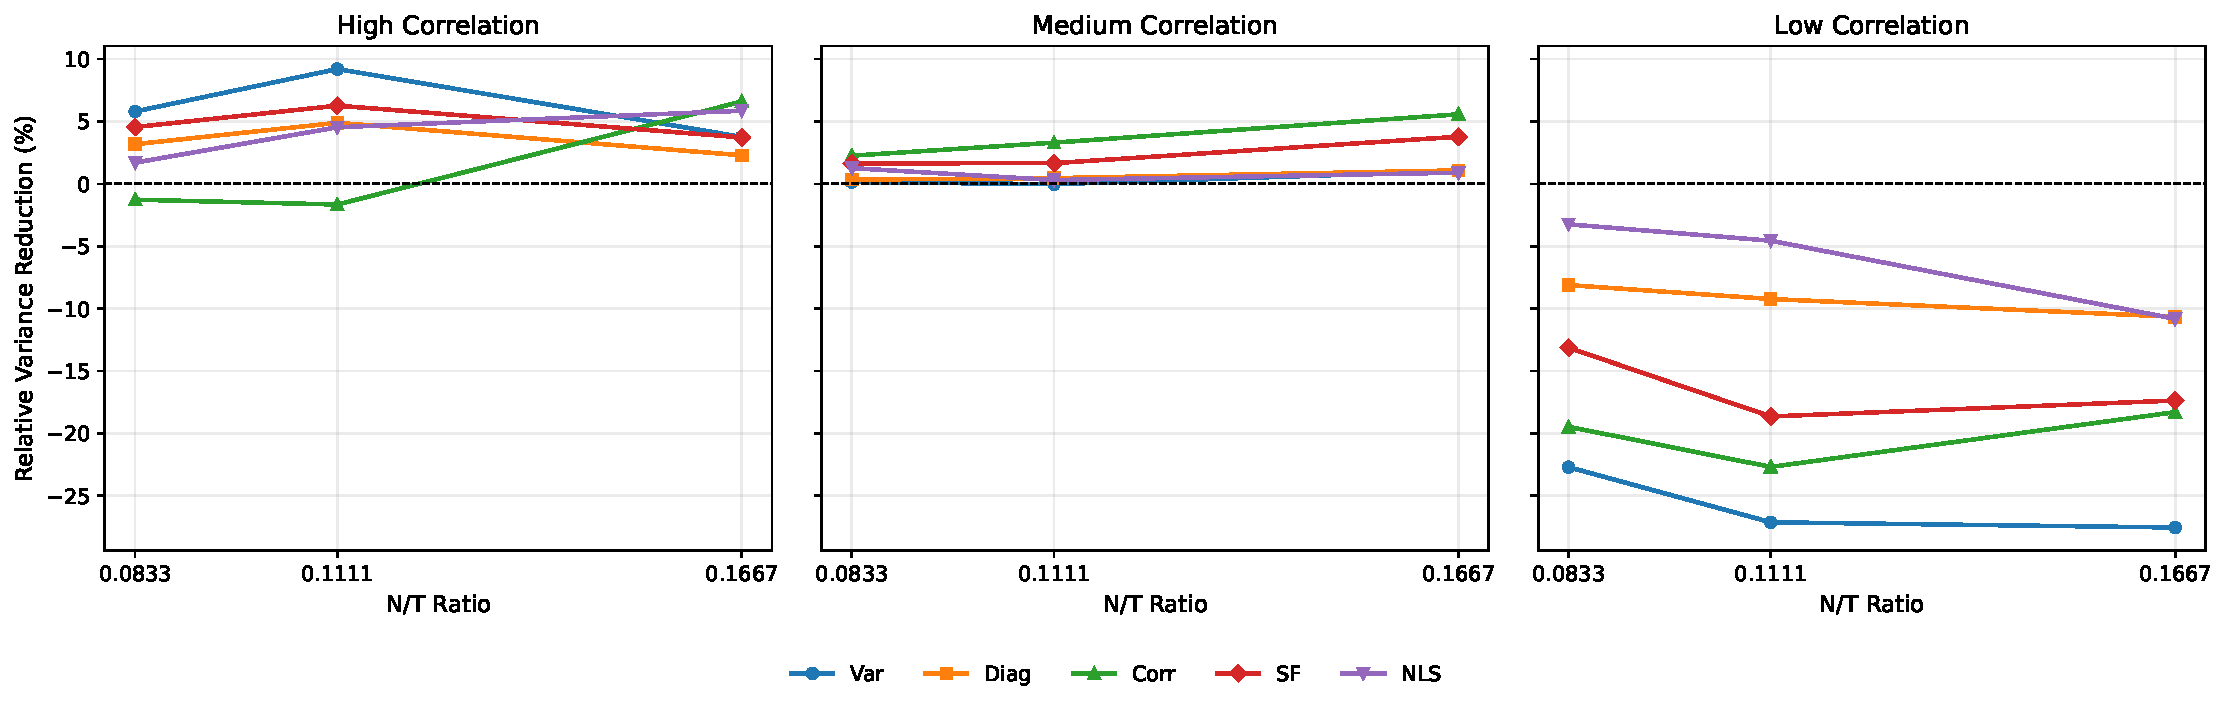
\includegraphics[width=\textwidth]
	{RVR_NT_Three_Portfolios.pdf}
	\caption{Корреляцын бүтэц ялгаатай гурван багцын
		$N/T$ харьцаанаас хамаарах RVR}
	\label{fig:nt_rvr_comparison}
\end{figure}

Зураг~\ref{fig:nt_rvr_comparison}-ээс харахад
High багцад Corr үнэлэгчээс бусад аргууд бүх
сургалтын цонхонд эерэг RVR үзүүлсэн боловч
хамгийн сайн үнэлэгч $N/T$ харьцаанаас
хамааран өөрчлөгдөж байна. Medium багцад
RVR-ийн хэмжээ харьцангуй бага бөгөөд
Corr үнэлэгч бүх цонхонд хамгийн өндөр
дисперсийн бууралт үзүүлэв. Харин Low
багцад бүх агшилтын үнэлэгчийн RVR сөрөг байгаа нь
Sample арга бүх цонхонд хамгийн бага
OOS дисперстэй байсныг харуулна.

Ийнхүү агшилтын үнэлэгчдийн гүйцэтгэл
корреляцийн бүтэц болон сургалтын цонхны
уртаас хамааран ялгаатай байна.
Гэхдээ $T$-г өөрчлөхөд сургалтын өгөгдлийн
хугацаа давхар өөрчлөгдөх тул ажиглагдсан
ялгааг зөвхөн $N/T$ харьцааны нөлөө
гэж тайлбарлах боломжгүй.


\paragraph{Мэдрэмжийн шинжилгээний HAC шалгалт.}

Багц тус бүрийн 15 харьцуулалтад
Holm-ийн засвар хэрэглэв.

\begin{table}[htbp]
	\centering
	\caption{Мэдрэмжийн шинжилгээний HAC шалгалт}
	\label{tab:nt_hac_summary}
	\small
	\begin{tabular}{lrlrr}
		\hline
		Багц & $T$ & Үнэлэгч & HAC $p$ & Holm $p$\\
		\hline
		High   & 90  & Diag & 0.0189 & 0.2839\\
		Medium & 90  & Corr & 0.1860 & 1.0000\\
		Low    & 120 & Corr & 0.0100 & 0.1504\\
		\hline
	\end{tabular}
\end{table}

\noindent
\textit{Тайлбар:} Багц тус бүрийн хамгийн
бага засварлаагүй $p$-утгатай хувилбарыг
үзүүлэв.

Holm-ийн засварыг хэрэглэсний дараа 5\%-ийн ач холбогдлын түвшинд статистикийн ач холбогдолтой ялгаа тогтоогдоогүй нь ажиглагдсан гүйцэтгэлийн зөрүүг агшилтын үнэлэгчдийн түүврийн ковариацын аргаас давуу эсвэл сул байгааг нотлох хангалттай статистик үндэслэл гэж үзэх боломжгүйг харуулж байна.

% --------------------------------------------------
\subsection{150 багцын robustness шинжилгээ}
\label{subsec:robustness_results}
% --------------------------------------------------

Үр дүн багцын бүрэлдэхүүнээс хамаарах
эсэхийг шалгах зорилгоор High, Medium,
Low ангилал тус бүрээс 50, нийт 150
багцад шинжилгээг давтав. Ангиллуудын
сургалтын хугацааны дундаж корреляц
харгалзан 0.5267, 0.3036, 0.1346 байв.

\begin{table}[htbp]
	\centering
	\caption{150 багцын дундаж RVR болон эерэг RVR-ийн хувь}
	\label{tab:robustness_rvr}
	\small
	\begin{tabular}{llrr}
		\hline
		Ангилал & Үнэлэгч &
		Дундаж RVR (\%) & Эерэг RVR (\%)\\
		\hline
		High & Var  & 1.13 & 72\\
		& Diag & 0.81 & 82\\
		& Corr & 0.65 & 60\\
		& SF   & 0.53 & 74\\
		& NLS  & 0.39 & 66\\
		\hline
		Medium & Var  & -1.31 & 48\\
		& Diag & 0.57 & 68\\
		& Corr & 0.55 & 54\\
		& SF   & 0.67 & 64\\
		& NLS  & 0.37 & 56\\
		\hline
		Low & Var  & -35.02 & 28\\
		& Diag & -0.61 & 54\\
		& Corr & 0.16 & 64\\
		& SF   & -1.36 & 42\\
		& NLS  & 0.99 & 74\\
		\hline
	\end{tabular}
\end{table}

High ангилалд бүх агшилтын үнэлэгчийн
дундаж RVR эерэг байна. Medium ангилалд
Var-аас бусад үнэлэгчдийн дундаж RVR
эерэг боловч бууралтын хэмжээ бага байв.

Low ангилалд Var үнэлэгчийн дундаж
RVR -35.02\% байгаа бол NLS үнэлэгчийнх
0.99\% байна. Иймээс анхны Low багцад
бүх агшилтын үнэлэгчийн RVR сөрөг
гарсан үр дүн нэмэлт 50 багцад
бүрэн давтагдсангүй.

% --------------------------------------------------
\subsection{Bootstrap итгэх завсар}
\label{subsec:bootstrap_results}
% --------------------------------------------------

Ангилал тус бүрийн дундаж RVR-ийн
тодорхой бус байдлыг зургаан сарын
блоктой, 3000 давталт бүхий circular
moving-block bootstrap аргаар үнэлэв.

\begin{table}[htbp]
	\centering
	\caption{Дундаж RVR-ийн 95\%-ийн bootstrap итгэх завсар}
	\label{tab:bootstrap_rvr}
	\small
	\begin{tabular}{llrrr}
		\hline
		Ангилал & Үнэлэгч &
		RVR (\%) & Доод & Дээд\\
		\hline
		High & Var  & 1.13 & -1.16 & 3.38\\
		& Diag & 0.81 & -0.09 & 1.83\\
		& Corr & 0.65 & -1.83 & 3.45\\
		& SF   & 0.53 & -0.54 & 1.55\\
		& NLS  & 0.39 & -0.45 & 1.40\\
		\hline
		Medium & Var  & -1.31 & -5.08 & 2.55\\
		& Diag & 0.57 & -0.67 & 1.87\\
		& Corr & 0.55 & -0.96 & 1.85\\
		& SF   & 0.67 & -0.39 & 1.46\\
		& NLS  & 0.37 & -0.66 & 1.45\\
		\hline
		Low & Var  & -35.02 & -65.61 & -14.67\\
		& Diag & -0.61 & -5.21 & 3.58\\
		& Corr & 0.16 & -1.95 & 2.15\\
		& SF   & -1.36 & -5.58 & 1.76\\
		& NLS  & 0.99 & -0.52 & 2.41\\
		\hline
	\end{tabular}
\end{table}

Low ангиллын Var үнэлэгчээс бусад
бүх үнэлэгчийн 95\%-ийн итгэх завсар
тэгийг агуулж байна. Харин Low
ангиллын Var үнэлэгчийн итгэх завсар
$[-65.61,-14.67]$ байгаа нь Sample
аргатай харьцуулахад дундаж OOS
дисперс өссөнийг дэмжиж байна.

Иймээс 150 багцын robustness шинжилгээний үр дүнгээр агшилтын үнэлэгчид Sample аргатай харьцуулахад OOS дисперсийг статистикийн хувьд ач холбогдолтойгоор бууруулдаг гэсэн хангалттай нотолгоо тогтоогдсонгүй. Харин Low ангиллын Var үнэлэгчийн дундаж RVR-ийн итгэх завсар тэгийг агуулаагүй бөгөөд энэ нь тухайн ангилалд дисперс өсөх хандлага ажиглагдсаныг илэрхийлнэ. Гэвч уг итгэх завсарт олон харьцуулалтын засвар хийгдээгүй тул энэ үр дүнг олон үнэлэгч, ангиллыг хамарсан статистик дүгнэлтийн түвшинд баталгаатай гэж үзэх боломжгүй.

% --------------------------------------------------
\subsection{Корреляцийн ангилал хоорондын харьцуулалт}
\label{subsec:tier_comparison_results}
% --------------------------------------------------

Агшилтын үнэлэгчдийн дундаж RVR
корреляцийн ангиллаас хамааран ялгаатай
эсэхийг шалгах зорилгоор High--Medium,
High--Low болон Medium--Low гэсэн гурван
хос харьцуулалт хийв. Ангилал бүрд таван
агшилтын үнэлэгчийг авч үзсэн тул нийт
15 харьцуулалт хийгдсэн.

Ангилал хоорондын дундаж RVR-ийн ялгааг
ижил сарын индексүүдээр гүйцэтгэсэн
circular moving-block bootstrap аргаар
үнэлж, 95\%-ийн итгэх завсрыг тооцсон.
Олон харьцуулалтаас үүдэх алдааг
хянахын тулд нийт 15 харьцуулалтын
$p$-утгад Holm-ийн засвар хэрэглэв.

\begin{table}[htbp]
	\centering
	\caption{Корреляцийн ангилал хоорондын
		дундаж RVR-ийн ялгааны bootstrap шинжилгээ}
	\label{tab:tier_comparison}
	\small
	\begin{tabular}{llrrrr}
		\hline
		Харьцуулалт & Үнэлэгч &
		Ялгаа &
		95\% CI доод &
		95\% CI дээд &
		Holm $p$\\
		\hline
		High--Medium
		& Var  &  2.43 & -0.57 &  5.46 & 1.000\\
		& Diag &  0.24 & -0.60 &  1.10 & 1.000\\
		& Corr &  0.10 & -2.62 &  3.32 & 1.000\\
		& SF   & -0.14 & -1.36 &  1.46 & 1.000\\
		& NLS  &  0.02 & -0.95 &  1.07 & 1.000\\
		\hline
		High--Low
		& Var  & 36.15 & 16.55 & 66.37 & 0.220\\
		& Diag &  1.42 & -2.03 &  5.45 & 1.000\\
		& Corr &  0.49 & -1.57 &  2.51 & 1.000\\
		& SF   &  1.89 & -1.67 &  6.82 & 1.000\\
		& NLS  & -0.60 & -1.71 &  0.81 & 1.000\\
		\hline
		Medium--Low
		& Var  & 33.71 & 15.23 & 63.54 & 0.252\\
		& Diag &  1.18 & -1.79 &  4.61 & 1.000\\
		& Corr &  0.39 & -2.45 &  2.81 & 1.000\\
		& SF   &  2.03 & -0.79 &  5.51 & 1.000\\
		& NLS  & -0.62 & -1.38 &  0.18 & 1.000\\
		\hline
	\end{tabular}
\end{table}

\noindent
\textit{Тайлбар:}
Ялгааг эхний ангиллын дундаж RVR-ээс
хоёр дахь ангиллын дундаж RVR-ийг
хасаж тооцсон. RVR-ийн ялгаа болон
итгэх завсрын хязгааруудыг процентын
пунктээр илэрхийлэв.
95\%-ийн итгэх завсрууд нь олон
харьцуулалтын засвар хийгдээгүй
bootstrap итгэх завсар бөгөөд
сүүлийн баганад 15 харьцуулалтад
Holm-ийн засвар хэрэглэсэн
$p$-утгуудыг харуулав.

Хүснэгт~\ref{tab:tier_comparison}-ээс
харахад High--Medium харьцуулалтад
Var үнэлэгчийн дундаж RVR-ийн ялгаа
2.43 процентын пункт байгаа бол
бусад үнэлэгчдийн ялгаа харьцангуй
бага байна. Гэхдээ таван үнэлэгчийн
бүх итгэх завсар тэгийг агуулж,
Holm-ийн засварласан $p$-утгууд
1.000 гарсан тул эдгээр хоёр
ангиллын хооронд статистикийн
ач холбогдолтой ялгаа тогтоогдсонгүй.

Харин High--Low болон Medium--Low
харьцуулалтад Var үнэлэгчийн
дундаж RVR-ийн ялгаа харгалзан
36.15 болон 33.71 процентын пункт
байна. Эдгээр ялгааны засварлаагүй
95\%-ийн bootstrap итгэх завсар
харгалзан [16.55, 66.37] болон
[15.23, 63.54] байгаа нь
хоёулаа тэгийг агуулаагүй.
Энэ нь засварлаагүй шинжилгээний
түвшинд Var үнэлэгчийн дундаж
RVR Low ангилалд High болон
Medium ангиллаас бага байгааг
илэрхийлж байна.

Гэвч олон харьцуулалтын засвар
хэрэглэсний дараа эдгээр хоёр
харьцуулалтын $p$-утга харгалзан
0.220 болон 0.252 болж,
5\%-ийн ач холбогдлын түвшнээс
давсан байна. Иймээс засварлаагүй
итгэх завсрууд тэгийг агуулаагүй
боловч олон харьцуулалтыг
хамтад нь авч үзэхэд эдгээр
ялгааг статистикийн хувьд
ач холбогдолтой гэж дүгнэх
хангалттай үндэслэлгүй байна.

Бусад дөрвөн үнэлэгчийн хувьд
High--Low болон Medium--Low
харьцуулалтын бүх итгэх завсар
тэгийг агуулж байна. Тухайлбал,
NLS үнэлэгчийн High--Low болон
Medium--Low ялгаа харгалзан
-0.60, -0.62 процентын пункт
байгаа боловч эдгээр ялгаа
статистикийн хувьд ач
холбогдолтой биш байна.

Ерөнхийд нь дүгнэвэл,
корреляцийн ангиллуудын хооронд
агшилтын үнэлэгчдийн дундаж
RVR-ийн ялгаа ажиглагдсан
боловч нийт 15 харьцуулалтад
Holm-ийн засвар хэрэглэсний
дараа 5\%-ийн түвшинд
статистикийн ач холбогдолтой
ялгаа тогтоогдсонгүй.
Иймээс корреляцийн ангиллаас
хамааран агшилтын үнэлэгчдийн
гүйцэтгэл ялгаатай байж болох
шинж тэмдэг ажиглагдсан ч
энэхүү ялгааг статистикийн
хувьд баталгаатай гэж
дүгнэх боломжгүй байна.


% --------------------------------------------------
\subsection{Тэнцүү жинтэй багцтай харьцуулалт}
\label{subsec:equal_weight_results}
% --------------------------------------------------

Ковариацын үнэлэгчид суурилсан GMVP-ийн
практик гүйцэтгэлийг үнэлэхийн тулд
хөрөнгө тус бүрд $1/N$ жин оноож,
сар бүр дахин тэнцвэржүүлдэг жишиг
багцтай харьцуулав. Бүх стратегид
үндсэн шинжилгээтэй ижил 52 сарын
OOS хугацааг ашиглав.

\begin{table}[htbp]
	\centering
	\caption{GMVP болон $1/N$ багцын OOS гүйцэтгэл ($T=120$)}
	\label{tab:equal_weight_comparison}
	\small
	\begin{tabular}{llrrr}
		\hline
		Багц & Стратеги &
		Жилийн хэлбэлзэл (\%) &
		$1/N$-тэй харьцуулсан RVR (\%) &
		Sharpe \\
		\hline
		High & Sample & 17.05 & 35.89 & 0.788 \\
		& Var & 16.55 & 39.61 & 0.843 \\
		& Diag & 16.78 & 37.93 & 0.816 \\
		& Corr & 17.16 & 35.08 & 0.821 \\
		& SF & 16.66 & 38.81 & 0.819 \\
		& NLS & 16.90 & 36.98 & 0.801 \\
		& $1/N$ & 21.29 & 0.00 & 0.840 \\
		\hline
		Medium & Sample & 14.28 & 15.72 & 0.601 \\
		& Var & 14.27 & 15.85 & 0.612 \\
		& Diag & 14.26 & 16.02 & 0.603 \\
		& Corr & 14.12 & 17.63 & 0.555 \\
		& SF & 14.16 & 17.11 & 0.577 \\
		& NLS & 14.19 & 16.79 & 0.603 \\
		& $1/N$ & 15.56 & 0.00 & 0.602 \\
		\hline
		Low & Sample & 13.77 & 26.06 & 0.269 \\
		& Var & 15.26 & 9.28 & 0.393 \\
		& Diag & 14.32 & 20.07 & 0.255 \\
		& Corr & 15.05 & 11.67 & 0.111 \\
		& SF & 14.65 & 16.36 & 0.190 \\
		& NLS & 13.99 & 23.67 & 0.313 \\
		& $1/N$ & 16.02 & 0.00 & 0.573 \\
		\hline
	\end{tabular}
\end{table}

Энэ хүснэгтийн RVR-ийг Sample бус, $1/N$
жишиг багцын дисперстэй харьцуулан тооцсон.
Хүснэгт~\ref{tab:equal_weight_comparison}-ээс
харахад гурван багцын хувьд зургаан GMVP
стратеги бүгд $1/N$ жишиг багцаас
бага OOS хэлбэлзэлтэй байна.
$1/N$ багцын жилийн хэлбэлзэл High,
Medium, Low багцад харгалзан
21.29\%, 15.56\%, 16.02\% байв.
Харин хамгийн бага хэлбэлзэлтэй
GMVP стратегиуд нь High багцад Var
(16.55\%), Medium багцад Corr (14.12\%),
Low багцад Sample (13.77\%) байна.

Гэхдээ хэлбэлзлийн давуу байдал нь
Sharpe-ийн харьцаагаар давуу байна
гэсэн үг биш. Тухайлбал, Low багцад
$1/N$ стратегийн Sharpe 0.573 байхад
GMVP стратегиудын Sharpe 0.111--0.393
хооронд байна. Иймээс GMVP-ийн
эрсдэлийг бууруулах зорилгыг
өгөөж--эрсдэлийн харьцааны үнэлгээнээс
тусад нь авч үзэх шаардлагатай.

% --------------------------------------------------
\subsection{Арилжааны зардлын нөлөө}
\label{subsec:trading_cost_results}
% --------------------------------------------------

Сар бүрийн дахин тэнцвэржүүлэлтийн
арилжааны зардлыг тооцохдоо нэг талын
арилжаанд 0, 5, 10, 25 суурь нэгж
(basis points, bps)-ийн хувилбаруудыг
ашиглав. Эхний OOS багц бүрдүүлэлтийн
зардлыг тооцоогүй. Доорх хүснэгтэд
нэг талын 10 bps зардлын хувилбарын
үр дүнг үзүүлэв.

\begin{table}[htbp]
	\centering
	\caption{Нэг талын 10 bps арилжааны зардлын дараах OOS гүйцэтгэл}
	\label{tab:trading_cost_results}
	\small
	\begin{tabular}{llrr}
		\hline
		Багц & Стратеги &
		Цэвэр Sharpe &
		Хуримтлагдсан цэвэр өгөөж (\%) \\
		\hline
		High & Sample & 0.784 & 67.46 \\
		& Var & 0.840 & 71.91 \\
		& Diag & 0.812 & 69.65 \\
		& Corr & 0.818 & 72.27 \\
		& SF & 0.816 & 69.53 \\
		& NLS & 0.797 & 68.45 \\
		& $1/N$ & 0.837 & 96.05 \\
		\hline
		Medium & Sample & 0.596 & 38.36 \\
		& Var & 0.607 & 39.31 \\
		& Diag & 0.599 & 38.56 \\
		& Corr & 0.551 & 34.21 \\
		& SF & 0.573 & 36.15 \\
		& NLS & 0.599 & 38.40 \\
		& $1/N$ & 0.599 & 42.07 \\
		\hline
		Low & Sample & 0.264 & 12.35 \\
		& Var & 0.388 & 22.92 \\
		& Diag & 0.251 & 11.77 \\
		& Corr & 0.107 & 2.13 \\
		& SF & 0.186 & 7.48 \\
		& NLS & 0.308 & 15.57 \\
		& $1/N$ & 0.568 & 40.28 \\
		\hline
	\end{tabular}
\end{table}

Арилжааны зардлыг тусгахад стратегиудын
Sharpe-ийн харьцаа зардалгүй
хувилбартай харьцуулахад бага зэрэг
буурч байна. Тухайлбал, High багцад
Var стратегийн Sharpe 0.843-аас
0.840 болж буурсан. Medium багцад
Var стратегийн цэвэр Sharpe 0.607,
Low багцад $1/N$ стратегийнх 0.568 байна.

High багцад $1/N$ стратегийн
хуримтлагдсан цэвэр өгөөж 96.05\%
байхад Var стратегийнх 71.91\% байна.
Иймээс GMVP стратегиудын хэлбэлзэл
бага байгаа нь хуримтлагдсан өгөөж
өндөр байна гэсэн баталгаа биш.
Эдгээр дүгнэлт нь сонгосон зардлын
хувилбар, сарын дахин тэнцвэржүүлэлт
болон 52 сарын OOS хугацаанд хамаарна.

% --------------------------------------------------
\subsection{GMVP ба $1/N$ багцын bootstrap харьцуулалт}
\label{subsec:bootstrap_equal_weight_results}
% --------------------------------------------------

GMVP стратегиудын $1/N$ жишиг багцтай
харьцуулсан дисперсийн бууралтын
тодорхой бус байдлыг 52 сарын OOS
өгөөжид суурилсан, зургаан сарын
блоктой, 3000 давталт бүхий circular
moving-block bootstrap аргаар үнэлэв.
Сар бүрийн индексүүдийг харьцуулж буй
стратегиудад ижил сонгож,
95\%-ийн percentile итгэх завсар
байгуулав. Багц тус бүрийн зургаан
харьцуулалтын bootstrap $p$-утгад
Holm-ийн засвар хэрэглэв.

\begin{table}[htbp]
	\centering
	\caption{GMVP-ийн $1/N$-тэй харьцуулсан RVR ба bootstrap шалгалт}
	\label{tab:bootstrap_equal_weight}
	\small
	\begin{tabular}{llrrrr}
		\hline
		Багц & Стратеги & RVR (\%) &
		95\% CI доод & 95\% CI дээд & Holm $p$ \\
		\hline
		High & Sample & 35.89 & -21.61 & 63.60 & 0.3149 \\
		& Var & 39.61 & -7.09 & 62.44 & 0.2639 \\
		& Diag & 37.93 & -15.32 & 64.14 & 0.3149 \\
		& Corr & 35.08 & -38.50 & 69.33 & 0.3149 \\
		& SF & 38.81 & -15.41 & 64.90 & 0.3149 \\
		& NLS & 36.98 & -16.53 & 62.84 & 0.3149 \\
		\hline
		Medium & Sample & 15.72 & -4.31 & 31.44 & 0.3399 \\
		& Var & 15.85 & -2.62 & 30.02 & 0.3399 \\
		& Diag & 16.02 & -3.31 & 31.15 & 0.3399 \\
		& Corr & 17.63 & -3.95 & 34.33 & 0.3399 \\
		& SF & 17.11 & -4.21 & 33.32 & 0.3399 \\
		& NLS & 16.79 & -3.61 & 31.72 & 0.3399 \\
		\hline
		Low & Sample & 26.06 & -7.84 & 51.16 & 0.5498 \\
		& Var & 9.28 & -16.30 & 29.00 & 0.8144 \\
		& Diag & 20.07 & -9.26 & 42.20 & 0.5498 \\
		& Corr & 11.67 & -20.01 & 35.14 & 0.8144 \\
		& SF & 16.36 & -18.68 & 40.65 & 0.8107 \\
		& NLS & 23.67 & -8.70 & 47.86 & 0.5498 \\
		\hline
	\end{tabular}
\end{table}

Хүснэгт~\ref{tab:bootstrap_equal_weight}-д
бүх GMVP стратегийн RVR эерэг байна.
Хамгийн бага хэлбэлзэлтэй стратегиудын
$1/N$-тэй харьцуулсан RVR нь High
багцад Var 39.61\%, Medium багцад
Corr 17.63\%, Low багцад Sample
26.06\% байна. Гэвч эдгээрийн
95\%-ийн итгэх завсар харгалзан
$[-7.09,62.44]$, $[-3.95,34.33]$,
$[-7.84,51.16]$ тул тэгийг агуулж байна.

Мөн багц тус бүрийн зургаан
харьцуулалтад Holm-ийн засвар
хэрэглэсний дараа 5\%-ийн түвшинд
статистикийн ач холбогдолтой ялгаа
илрээгүй. Bootstrap $p$-утгыг
төвлөрүүлсэн bootstrap тархалтаас,
харин итгэх завсрыг percentile
аргаар байгуулсан тул засварлаагүй
$p$-утга ба итгэх завсрын шийдвэр
зарим тохиолдолд зөрж болохыг
харгалзан үзнэ. Иймээс ажиглагдсан
эерэг RVR-ийг статистикийн хувьд
баталгаатай давуу байдал гэж
тайлбарлахгүй.

% --------------------------------------------------
\subsection{Үр дүнгийн нэгтгэл}
\label{subsec:results_summary}
% --------------------------------------------------

Эмпирик шинжилгээгээр ковариацын
матрицын агшилтын үнэлэгчдийн
гүйцэтгэл багцын бүрэлдэхүүн болон
сургалтын цонхны уртаас хамааран
ялгаатай байгааг ажиглав.

Анхны гурван багцын HAC шалгалт
болон 150 багцын bootstrap шинжилгээ
нь агшилтын үнэлэгчдийн Sample
аргаас тогтвортой давуу байдлыг
статистикийн хувьд батлаагүй.

Харин бага корреляцтай багцуудад
Var үнэлэгчийн дундаж RVR
мэдэгдэхүйц сөрөг гарсан нь
агшилтын арга бүр OOS эрсдэлийг
бууруулах баталгаагүйг харуулж байна.

Ангилал хоорондын харьцуулалтаар
ажиглагдсан ялгаа олон шалгалтын
засварын дараа статистикийн
ач холбогдолтой болох нь
тогтоогдсонгүй.

$1/N$ жишиг багцтай харьцуулахад
зургаан GMVP стратеги гурван багцад
бүгд бага OOS хэлбэлзэлтэй байсан
боловч bootstrap шалгалтын
олон харьцуулалтын засварын дараа
статистикийн ач холбогдолтой давуу
байдал тогтоогдсонгүй. Мөн
арилжааны зардлыг тооцоход
стратегиудын цэвэр гүйцэтгэл
буурч, хэлбэлзлийн давуу байдал
Sharpe болон хуримтлагдсан
өгөөжийн давуу байдалтай
заавал давхцахгүй байв.

Ковариацын үнэлэгчдийн хоорондын OOS хэлбэлзлийн
ялгаа олон тохиолдолд бага байгаа нь long-only
хязгаарлалттай багцад нэмэлт агшилтын үр ашиг
хязгаарлагдаж болохыг харуулсан
\citet{DeNardKostovic2026}-ийн үр дүнтэй
нийцэж байна. Тэдний судалгаанд багцын жингийн
хязгаарлалт нь өөрөө зохицуулах нөлөө үзүүлж,
ковариацын матрицад нэмэлт агшилт хийх хэрэгцээг
бууруулж болохыг авч үзсэн. Гэхдээ уг судалгаанд
өдрийн өгөөж, илүү олон хөрөнгөтэй багцуудыг
шинжилсэн бол энэхүү судалгаанд зөвхөн сарын
өгөөж, бага $N/T$ харьцаатай 10 хөрөнгийн
багцуудыг ашигласан. Иймээс хоёр судалгааны
үр дүнг шууд ижил нөхцөлийн нотолгоо гэж үзэхгүй.



\section{Дүгнэлт}
\label{sec:conclusion}

Энэхүү судалгаагаар хөрөнгийн тоо болон сургалтын ажиглалтын
тооны харьцаа ($N/T$) бага нөхцөлд ковариацын матрицын
агшилтын үнэлэгчдийн глобал хамгийн бага вариацтай багц
(GMVP)-ын оновчлол дахь гүйцэтгэлийг харьцуулан шинжиллээ.
Түүврийн ковариацын матриц (Sample), тогтмол вариацын (Var),
диагональ (Diag), тогтмол корреляцын (Corr), нэг хүчин зүйлийн
(SF) зорилтот матрицад суурилсан шугаман агшилтын үнэлэгчид
болон шугаман бус агшилтын үнэлэгчийг (NLS) авч үзэв.
Корреляцын бүтэц ялгаатай, тус бүр 10 хувьцаанаас бүрдсэн
гурван багцад богино борлуулалтыг зөвшөөрөөгүй GMVP
байгуулж, 120 сарын сургалтын цонх болон 52 сарын
түүврээс гадуурх (OOS) хугацаанд үнэлэв.

Үндсэн шинжилгээнд агшилтын үнэлэгчдийн гүйцэтгэл
багцын корреляцын бүтцээс хамааран ялгаатай байв.
Өндөр корреляцтай багцад Var үнэлэгч Sample аргатай
харьцуулахад OOS дисперсийг 5.81\%-иар, дунд
корреляцтай багцад Corr үнэлэгч 2.26\%-иар
бууруулсан. Харин бага корреляцтай багцад Sample
арга хамгийн бага OOS дисперстэй байсан бөгөөд
агшилтын таван үнэлэгчийн харьцангуй дисперсийн
бууралт (RVR) бүгд сөрөг гарсан. Иймээс нэг
үнэлэгч бүх багцад тогтмол давуу гүйцэтгэл
үзүүлээгүй.

Багцын жингийн шинжилгээгээр Corr үнэлэгч
гурван багцад хамгийн бага дундаж turnover,
Var үнэлэгч хамгийн бага дундаж HHI үзүүлсэн.
Гэвч жингийн эргэлт болон төвлөрөл бага байх
нь OOS дисперс заавал бага байхыг илэрхийлээгүй.
Тухайлбал, бага корреляцтай багцад Var
үнэлэгч хамгийн бага HHI-тэй боловч OOS
дисперс нь Sample аргынхаас 22.70\%-иар
өндөр байв.

Сургалтын цонхны уртыг 60, 90 болон 120 сар
болгон өөрчилсөн мэдрэмжийн шинжилгээнд
үнэлэгчдийн гүйцэтгэлийн эрэмбэ бүх багцад
тогтвортой хадгалагдсангүй. Өндөр корреляцтай
багцад хамгийн өндөр RVR үзүүлсэн үнэлэгч
сургалтын цонхноос хамааран өөрчлөгдсөн бол
дунд корреляцтай багцад Corr үнэлэгч,
бага корреляцтай багцад Sample арга бүх
цонхонд хамгийн бага OOS дисперстэй байв.
Иймээс $N/T$ харьцаа буурах тусам агшилтын
аргуудын давуу тал заавал нэмэгдэнэ гэсэн
зүй тогтол ажиглагдсангүй.

Үндсэн гурван багцын сарын квадрат өгөөжийн
ялгаанд хийсэн HAC шалгалтаар Holm-ийн
засварын дараа 5\%-ийн түвшинд статистикийн
ач холбогдолтой ялгаа илрээгүй. Сургалтын
цонхны мэдрэмжийн шинжилгээнд мөн ижил
үр дүн гарсан. Эдгээр шалгалт нь квадрат
өгөөжийн дундаж ялгаанд суурилсан тул
OOS дисперсийн ялгааг шууд шалгасан гэж
үзэхгүй.

Үр дүн багцын бүрэлдэхүүнээс хамаарах
эсэхийг үнэлэхийн тулд корреляцын ангилал
тус бүрээс 50, нийт 150 нэмэлт багцад
шинжилгээг давтав. Өндөр корреляцтай
ангилалд агшилтын бүх үнэлэгчийн дундаж
RVR эерэг байсан бол дунд болон бага
корреляцтай ангиллуудад үр дүн харилцан
адилгүй байв. Ялангуяа бага корреляцтай
ангилалд Var үнэлэгчийн дундаж RVR
$-35.02\%$, харин NLS үнэлэгчийнх
$0.99\%$ байв. Иймээс анхны бага
корреляцтай багцад бүх агшилтын
үнэлэгчийн RVR сөрөг гарсан үр дүн
нэмэлт 50 багцад бүрэн давтагдсангүй.

Нэмэлт 150 багцын дундаж RVR-ийн
тодорхой бус байдлыг circular
moving-block bootstrap аргаар үнэлэхэд
бага корреляцтай ангиллын Var
үнэлэгчээс бусад бүх үнэлэгчийн
засварлаагүй 95\%-ийн итгэх завсар
тэгийг агуулсан. Бага корреляцтай
ангиллын Var үнэлэгчийн итгэх завсар
$[-65.61,-14.67]$ байв. Корреляцын
ангилал хоорондын харьцуулалтад
Var үнэлэгчийн High--Low болон
Medium--Low ялгааны засварлаагүй
bootstrap $p$-утга харгалзан
0.0147, 0.0180 байсан боловч
15 харьцуулалтад Holm-ийн засвар
хэрэглэсний дараа 0.2199, 0.2519
болсон. Иймээс ангилал хоорондын
ялгаа олон харьцуулалтын засварын
дараа статистикийн хувьд
батлагдсангүй.

Тэнцүү жинтэй $1/N$ багцыг нэмэлт
жишиг болгон авч үзэхэд үндсэн гурван
багцад ковариацын зургаан үнэлэгчид
суурилсан GMVP стратегиуд бүгд
$1/N$ багцаас бага OOS хэлбэлзэл
үзүүлсэн. Өндөр корреляцтай багцад
Var үнэлэгчийн $1/N$-тэй харьцуулсан
дисперсийн бууралт 39.61\%,
дунд корреляцтай багцад Corr
үнэлэгчийнх 17.63\%, бага
корреляцтай багцад Sample аргынх
26.06\% байв. Гэвч эрсдэлд
тохируулсан өгөөжийн хувьд
GMVP стратегиуд бүх нөхцөлд
давуу байгаагүй. Тухайлбал,
бага корреляцтай багцад
$1/N$ стратегийн жилийн
Sharpe-ийн харьцаа GMVP
стратегиудынхаас өндөр байв.

GMVP болон $1/N$ багцын OOS
дисперсийн харьцаанд хийсэн
circular moving-block bootstrap
шинжилгээгээр дээрх гурван
харьцуулалтын засварлаагүй
95\%-ийн итгэх завсар
харгалзан $[-7.09,62.44]$,
$[-3.95,34.33]$ болон
$[-7.84,51.16]$ байв.
Итгэх завсрууд тэгийг
агуулж, багц тус бүрийн
зургаан харьцуулалтад
Holm-ийн засвар хэрэглэсний
дараа статистикийн ач
холбогдолтой ялгаа
тогтоогдоогүй. Иймээс
GMVP стратегиуд $1/N$
багцаас бага OOS дисперстэй
байсан нь ажиглагдсан
үр дүн боловч статистикийн
хувьд тогтвортой давуу
байдлыг батлахад хангалтгүй
байна.

Арилжааны зардлын мэдрэмжийн
шинжилгээнд багцын дахин
тэнцвэржүүлэлттэй холбоотой
нэг талын 10 суурь нэгжийн
зардлыг тооцоход стратегиудын
Sharpe-ийн харьцаа бага
хэмжээгээр буурсан боловч
үндсэн харьцуулалтын ерөнхий
дүр зураг өөрчлөгдөөгүй.
Гэсэн хэдий ч хамгийн бага
дисперстэй стратеги нь
хамгийн өндөр хуримтлагдсан
өгөөжтэй байх албагүй.
Иймээс ковариацын үнэлэгчийн
практик үр ашгийг зөвхөн
OOS хэлбэлзлээр бус,
арилжааны зардлын дараах
гүйцэтгэлтэй хамтатган
үнэлэх шаардлагатай.

\paragraph{Практик ач холбогдол.}

Судалгааны үр дүн нь бага $N/T$
харьцаатай нөхцөлд ковариацын
матрицын агшилтыг түүврийн
ковариацын матрицаас үргэлж
давуу гэж үзэх үндэслэлгүйг
харуулж байна. Агшилтын
үнэлэгчдийн гүйцэтгэл багцын
корреляцын бүтэц, хөрөнгийн
бүрэлдэхүүн болон сургалтын
цонхны уртаас хамааран
өөрчлөгдөж байна.

Нөгөө талаас GMVP стратегиуд
тэнцүү жинтэй багцаас бага
OOS хэлбэлзэл үзүүлсэн нь
ковариацын матрицад суурилсан
оновчлол эрсдэлийг удирдахад
ашигтай байж болохыг харуулна.
Гэхдээ энэхүү ажиглагдсан
давуу тал статистикийн
хувьд батлагдаагүй бөгөөд
бага хэлбэлзэл нь өндөр
Sharpe-ийн харьцаа эсвэл
өндөр хуримтлагдсан өгөөжийг
заавал илэрхийлэхгүй.

Иймээс хөрөнгө оруулалтын
практикт ковариацын үнэлэгчийг
зөвхөн онолын шинж чанар
эсвэл агшилтын аргын төрлөөр
сонгохын оронд rolling-window
OOS шинжилгээгээр харьцуулж,
дисперс, жингийн эргэлт,
төвлөрөл, эрсдэлд тохируулсан
өгөөж болон арилжааны
зардлыг хамтад нь үнэлэх
нь зүйтэй. Мөн Sample болон
$1/N$ стратегийг харьцуулалтын
жишиг болгон ашиглах нь
оновчлолын болон агшилтын
аргын нэмэлт үр ашгийг
ялган үнэлэхэд чухал юм.

Энэхүү судалгааны үр дүн нь
сонгосон хувьцааны багцууд,
богино борлуулалтыг
зөвшөөрөөгүй оновчлол болон
52 сарын OOS хугацааны
хүрээнд хязгаарлагдана.
Багцуудыг бүрэн хугацааны
өгөгдөлтэй хувьцаануудаас
сонгосон нь сонголтын
хазайлт үүсгэх боломжтой.
Мөн сургалтын цонхны уртыг
өөрчлөхөд $N/T$ харьцаанаас
гадна сургалтын өгөгдлийн
хугацаа өөрчлөгдсөн.
Нэмэлт 150 багц нь бие
даасан санамсаргүй түүвэр
биш бөгөөд bootstrap
шинжилгээнд багцын
бүрэлдэхүүнийг тогтмол
гэж үзсэн. Түүнчлэн
арилжааны зардлын шинжилгээ
нь нэг талын тогтмол
зардлын таамаглалд
суурилсан бөгөөд зах
зээлийн нөлөөлөл болон
бусад бодит арилжааны
хязгаарлалтыг бүрэн
тусгаагүй.

Нэгдсэн дүнгээр бага $N/T$
харьцаатай нөхцөлд
ковариацын матрицын
агшилтын үнэлэгчид GMVP-ийн
OOS дисперсийг бууруулах
боломжтой боловч энэхүү
давуу тал нь бүх багц
болон үнэлэгчид тогтвортой
хадгалагдсангүй. Харин
GMVP стратегиудын $1/N$
багцаас бага хэлбэлзэлтэй
байсан үр дүн нь ковариацын
матрицад суурилсан
оновчлолын боломжит
ач холбогдлыг харуулж
байна. Гэвч статистикийн
шалгалтуудын олон
харьцуулалтын засварын
дараа агшилтын үнэлэгчдийн
Sample аргаас, мөн GMVP
стратегиудын $1/N$ багцаас
давуу гүйцэтгэлийг батлах
хангалттай нотолгоо
илрээгүй. Иймээс ковариацын
матрицын агшилтыг бага
$N/T$ нөхцөлд эрсдэлийг
заавал бууруулах арга бус,
харин багцын бүтэц,
түүврээс гадуурх гүйцэтгэл
болон практик зардалд
тулгуурлан үнэлэх
шаардлагатай хувилбар
гэж дүгнэв.



	% 7. DISCUSSION
	% ==================================================
	
% ==================================================
% CONCLUSION
% ==================================================


	% ==================================================
	% REFERENCES
	% ==================================================
	
	\bibliographystyle{plainnat}
	\bibliography{references}
	
\end{document}